\chapter{\texorpdfstring{$L$}{L}-functions}\label{ch:Standard_Class_L-functions}
  We start our discussion of $L$-functions with Dirichlet series. Dirichlet series are essential tools in analytic number theory because they are a way of analytically encoding arithmetic information. If the Dirichlet series possesses sufficiently large analytic continuation we call it an $L$-function and from the analytic properties of $L$-functions we can extract number theoritic results. After discussing Dirichlet series we will define a specific class of $L$-functions: Selberg class $L$-functions. Next we show that several natural Dirichlet series are actually Selberg class $L$-functions. Specifically, we discuss the Riemann zeta function, $L$-functions attached to Dirichlet characters, and $L$-functions formed from modular forms. In the case of modular forms we also describe a method of Rankin and Selberg for constructing new $L$-functions from old ones.
  \section{The General Setup for \texorpdfstring{$L$}{L}-functions}\label{sec:The_General_Setup_for_L-functions}
    \subsection*{Dirichlet Series}
      A \textbf{Dirichlet series}\index{Dirichlet series} $D(s)$ is a sum of the form
      \[
        D(s) = \sum_{n \ge 1}\frac{a(n)}{n^{s}},
      \]
      with $a(n) \in \C$. We exclude the case $a(n) = 0$ for all $n \ge 1$ so that $D(s)$ is not identically zero. We would first like to understand where this series converges. It does not take much for $D(s)$ to converge uniformly in a sector:

      \begin{theorem}\label{thm:convergence_of_Dirichlet_series}
        Suppose $D(s)$ is a Dirichlet series with coefficient $a(n)$ and that $D(s)$ converges at $s_{0} = \s_{0}+it_{0}$. Then for any $H > 0$, $D(s)$ converges uniformly in the sector
        \[
          \{s = \s+it \in \C:\s \ge \s_{0}, |t-t_{0}| \le H(\s-\s_{0})\}.
        \]
      \end{theorem}
      \begin{proof}
        Set $R(u) = \sum_{n \ge u}\frac{a(n)}{n^{-s_{0}}}$ so that $a(n) = (R(n)-R(n+1))n^{s_{0}}$. Then for any two positive integers $N$ and $M$ with $1 \le M < N$, partial summation (see \cref{append:Summation_Formulas}) implies
        \begin{equation}\label{equ:convergence_of_Dirichlet_series_1}
          \sum_{M \le n \le N}\frac{a(n)}{n^{s}} = R(M)M^{s_{0}-s}-R(N)N^{s_{0}-s}-\sum_{M+1 \le n \le N}R(n)((n-1)^{s_{0}-s}-n^{s_{0}-s}).
        \end{equation}
        We will now express the sum on the right-hand side as an integral. To do this, observe that
        \[
          (n-1)^{s_{0}-s}-n^{s_{0}-s} = -(s_{0}-s)\int_{n-1}^{n}u^{s_{0}-s-1}\,du.
        \]
        Therefore
        \begin{equation}\label{equ:convergence_of_Dirichlet_series_2}
          \begin{aligned}
            \sum_{M+1 \le n \le N}R(n)((n-1)^{s_{0}-s}-n^{s_{0}-s}) &= -(s_{0}-s)\sum_{M+1 \le n \le N}R(n)\int_{n-1}^{n}u^{s_{0}-s-1}\,du \\
            &= -(s_{0}-s)\sum_{M+1 \le n \le N}\int_{n-1}^{n}R(u)u^{s_{0}-s-1}\,du \\
            &= -(s_{0}-s)\int_{M}^{N}R(u)u^{s_{0}-s-1}\,du,
          \end{aligned}
        \end{equation}
        where the second to last line follows because $R(u)$ is constant on the interval $[u,u+1)$. Combining \cref{equ:convergence_of_Dirichlet_series_1,equ:convergence_of_Dirichlet_series_2} gives
        \begin{equation}\label{equ:convergence_of_Dirichlet_series_3}
          \sum_{M \le n \le N}\frac{a(n)}{n^{s}} = R(M)M^{s_{0}-s}-R(N)N^{s_{0}-s}+(s_{0}-s)\int_{M}^{N}R(u)u^{s_{0}-s-1}\,du.
        \end{equation}
        Now for any $\e > 0$ there exists an $M$ such that $|R(u)| < \e$ for all $u \ge M$ because $D(s)$ is convergent at $s_{0}$. In particular, $|R(u)u^{s_{0}-s}| < \e$ for all $u \ge M$ becuase $\s \ge \s_{0}$. Moreover for $s$ in the prescribed sector,
        \[
          |s-s_{0}| \le (\s-\s_{0})+|t-t_{0}| \le (H+1)(\s-\s_{0}).
        \]
        These estimates and \cref{equ:convergence_of_Dirichlet_series_3} together imply
        \[
          \left|\sum_{M \le n \le N}\frac{a(n)}{n^{s}}\right| = 2\e+\e|s-s_{0}|\int_{M}^{N}u^{\s_{0}-\s-1}\,du \le 2\e+\e(H+1)(\s-\s_{0})\int_{M}^{N}u^{\s_{0}-\s-1}\,du.
        \]
        Since the integral is finite, $\sum_{M \le n \le N}\frac{a(n)}{n^{s}}$ can be made arbitrarly small uniformly for $s$ in the desired sector. The claim now follows by the uniform version of Cauchy's criterion.
      \end{proof}
      
      By taking $H \to \infty$ in \cref{thm:convergence_of_Dirichlet_series} we see that $D(s)$ converges in the half-plane $\Re(s) > \s_{0}$. Moreover, since the terms of $D(s)$ are holomorphic, and the convergence is locally uniform (actually uniform in sectors), it follows that $D(s)$ is holomorphic in the region $\Re(s) > \Re(s_{0})$. Now let $\s_{c}$ be the infimum of all $\Re(s)$ for which $D(s)$ converges. We call $\s_{c}$ the \textbf{abscissa of convergence}\index{abscissa of convergence} of $D(s)$. Similarly, let $\s_{a}$ be the infimum of all $\Re(s)$ for which $D(s)$ converges absolutely and hence absolutely uniformly on compacta by the previous comment about locally uniform convergence. We call $\s_{a}$ the \textbf{abscissa of absolute convergence}\index{abscissa of absolute convergence} of $D(s)$. One should think of $\s_{c}$ and $\s_{a}$ as the boundaries of convergence and absolute convergence respectively. Of course, anything can happen at $\Re(s) = \s_{c}$ and $\Re(s) = \s_{a}$, but to the right of these lines we have convergence and absolute convergence of $D(s)$ respectively. It turns out that $\s_{a}$ is never far from $\s_{c}$ provided $\s_{c}$ is finite:

      \begin{theorem}
        If $D(s)$ is a Dirichlet series with finite abscissa of convergence $\s_{c}$, then
        \[
          \s_{c} \le \s_{a} \le \s_{c}+1.
        \]
      \end{theorem}
      \begin{proof}
        The first inequality is trivial since absolute convergence implies convergence. For the second inequality, let $\e > 0$. Since $D(s)$ converges at $\s_{c}+\e$, the terms $a(n)n^{-(\s_{c}+\e)}$ tend to zero as $n \to \infty$. Therefore $a(n) \ll_{\e} n^{\s_{c}+\e}$ where the implicit constant is independent of $n$. But then $a(n)n^{-(\s_{c}+\e)} \ll_{\e} 1$ which implies $\sum_{n \ge 1}a(n)n^{-(\s_{c}+1+2\e)}$ is absolutely convergent by the comparison test with respect to $\sum_{n \ge 1}n^{-(1+\e)}$. In terms of $D(s)$, this means $\s_{a} \le \s_{c}+1+2\e$ and taking $\e \to 0$ gives the second inequality.
      \end{proof}

      We will now introduce several convergence theorems for Dirichlet series. It will be useful to setup some notation first. If $D(s)$ is a Dirichlet series with coefficients $a(n)$, then for any real $X$ we set
      \[
        A(X) = \sum_{n \le X}a(n).
      \]
      This is the partial sum of the coefficients $a(n)$ up to $X$. Our first convergence theorem relates boundeness of $A(X)$ to the value of $\s_{c}$: 
      
      \begin{proposition}\label{prop:Dirichlet_series_convergence_bounded_coefficient_sum}
        Suppose $D(s)$ is a Dirichlet series and that $A(X) \ll 1$. Then $\s_{c} \le 0$.
      \end{proposition}
      \begin{proof}
        Fix $s$ be such that $\Re(s) > 0$. Since $A(X) \ll 1$, $A(X)X^{s} \to 0$ as $X \to \infty$. Abel's summation formula (see \cref{append:Summation_Formulas}) then implies
        \[
          D(s) = s\int_{1}^{\infty}A(u)u^{-(s+1)}\,du.
        \]
        But because $A(u) \ll 1$, we have
        \[
          s\int_{1}^{\infty}A(u)u^{-(s+1)}\,du \ll s\int_{1}^{\infty}u^{-(s+1)}\,du = -u^{-s}\big|_{1}^{\infty} = 1.
        \]
        Therefore the integral converges for $\Re(s) > 0$ and hence $D(s)$ does too. It follows that $\s_{c} \le 0$.
      \end{proof}

      Our next theorem states that if the coefficients of $D(s)$ are polynomially bounded, we can obtain an upper bound for the abscissa of absolute convergence:

      \begin{proposition}\label{prop:Dirichlet_series_convergence_polynomial_bound}
        Suppose $D(s)$ is a Dirichlet series whose coefficients $a(n)$ satisfy $|a(n)| \ll n^{\a}$ for some real $\a$. Then the abscissa of absolute convergence satisfies $\s_{a} \le 1+\a$.
      \end{proposition}
      \begin{proof}
        It suffices to show that $D(s)$ is absolutely convergent in the region $\Re(s) > 1+\a$. For $s$ is in this region, the polynomial bound gives
        \[
          |D(s)| \le \sum_{n \ge 1}\left|\frac{a(n)}{n^{s}}\right| \ll \sum_{n \ge 1}\frac{1}{n^{s-\a}}.
        \]
        The latter series converges by the integral test because $\Re(s)-\a > 1$. Therefore $D(s)$ is absolutely convergent.
      \end{proof}

      Obtaining polynomial bounds on coefficients of Dirichlet series are, in most cases, not hard to establish. So the assumption in \cref{prop:Dirichlet_series_convergence_polynomial_bound} is mild. Actually, there is a partial converse to \cref{prop:Dirichlet_series_convergence_polynomial_bound} which gives an approximate size to $A(X)$:

      \begin{proposition}\label{prop:Dirichlet_series_coefficient_size_on_average}
        Suppose $D(s)$ is a Dirichlet series with coefficients $a(n)$ and finite and non-negative abscissa of absolute convergence $\s_{a}$. Then for any $\e > 0$,
        \[
          A(X) \ll_{\e} X^{\s_{a}+\e}.
        \]
      \end{proposition}
      \begin{proof}
        By Abel's summation formula (see \cref{append:Summation_Formulas}),
        \begin{equation}\label{prop:Dirichlet_series_coefficient_size_on_average_1}
          \sum_{n \le X}\frac{a(n)}{n^{\s_{a}+\e}} = A(X)X^{-(\s_{a}+\e)}+(\s_{a}+\e)\int_{0}^{X}A(u)u^{-(\s_{a}+\e+1)}\,du.
        \end{equation}
        If we set $R(u) = \sum_{n \ge u}\frac{a(n)}{n^{\s_{a}+\e}}$, then $a(n) = (R(n)-R(n+1))n^{\s_{a}+\e}$ and it follows that
        \[
          A(u) = \sum_{n \le u}(R(n)-R(n+1))n^{\s_{a}+\e}.
        \]
        Substituting this into \cref{prop:Dirichlet_series_coefficient_size_on_average_1}, we obtain
        \[
          \int_{0}^{X}\sum_{n \le u}(R(n)-R(n+1))n^{\s_{a}+\e}u^{-(\s_{a}+\e+1)}\,du.
        \]
        As $R(n)$ is constant on the interval $[n,n+1)$, linearity of the integral implies
        \[
          \int_{0}^{X}\sum_{n \le u}(R(n)-R(n+1))n^{\s_{a}+\e}u^{-(\s_{a}+\e+1)}\,du = \sum_{0 \le n \le X}(R(n)-R(n+1))n^{\s_{a}+\e}\int_{n}^{n+1}u^{-(\s_{a}+\e+1)}+O_{\e}(1),
        \]
        where the $O$-estimate is present since $X$ may not be an integer. Now $R(n) \ll_{\e} 1$ since it is the tail of $D(\s_{a}+\e)$ and moreover,
        \[
          \int_{n}^{n+1}u^{-(\s_{a}+\e+1)} = -\frac{u^{-(\s_{a}+\e)}}{\s_{a}+\e}\bigg|_{n}^{n+1} = \frac{n^{-(\s_{a}+\e)}}{\s_{a}+\e}-\frac{(n+1)^{-(\s_{a}+\e)}}{\s_{a}+\e} \ll_{\e} 1,
        \]
        because $\s_{a}+\e > 0$. So
        \[
          \int_{0}^{X}A(u)u^{-(\s_{a}+\e+1)}\,du = \int_{0}^{X}\sum_{n \le u}(R(n)-R(n+1))n^{\s_{a}+\e}u^{-(\s_{a}+\e+1)}\,du \ll_{\e} 1.
        \]
        Also, $\sum_{n \le X}\frac{a(n)}{n^{\s_{a}+\e}} \ll_{\e} 1$ because $D(\s_{a}+\e)$ converges. We conclude
        \[
          A(X)X^{-(\s_{a}+\e)} = \sum_{n \le X}\frac{a(n)}{n^{\s_{a}+\e}}-(\s_{a}+\e)\int_{0}^{X}A(u)u^{-(\s_{a}+\e+1)}\,du. \ll_{\e} 1,
        \]
        which is equivalent to the desired estimate.
      \end{proof}

      A way to think about \cref{prop:Dirichlet_series_coefficient_size_on_average} is that if the abscissa of absolute convergence is $\s_{a} \ge 0$ then the size of the coefficients $a(n)$ is at most $n^{\s_{a}+\e}$ on average for any $\e > 0$. Of corse, if $a(n) \ll n^{\a}$ then \cref{prop:Dirichlet_series_convergence_polynomial_bound} implies that $\s_{a} \le 1+\a$ and so \cref{prop:Dirichlet_series_coefficient_size_on_average} gives the significantly weaker estimate $A(X) \ll_{\e} X^{1+\a+\e}$. However, if we only have a bound of the form $A(X) \ll X^{\a}$ we can still obtain an upper estimate for the abscissa of absolute convergence:

      \begin{proposition}\label{prop:Dirichlet_series_convergence_polynomial_bound_average}
        Suppose $D(s)$ is a Dirichlet series with coefficients $a(n)$ such that $A(X) \ll X^{\a}$ for some real $\a \ge 0$. Then the abscissa of absolute convergence satisfies $\s_{a} \le \a$.
      \end{proposition}
      \begin{proof}
        It suffices to show that $D(s)$ is absolutely convergent in the region $\Re(s) > \a$. Let $s$ be in this region and set $\Re(s) = \b$. Note that $\b > \a$. Then
        \[
          |D(s)| \le \sum_{n \ge 1}\left|\frac{a(n)}{n^{s}}\right| = \sum_{n \ge 1}\frac{|a(n)|}{n^{\b}}.
        \]
        By Abel's summation formula (see \cref{append:Summation_Formulas}),
        \[
          \sum_{n \le N}|a(n)|n^{-\b} = |a(N)|N^{-\b}-|a(1)|+\b\int_{1}^{N}A^{\ast}(u)u^{-(\b+1)}\,du,
        \]
        where $A^{\ast}(u) = \sum_{n \le u}|a(n)|$. Now $A(u) \ll u^{\a}$, which is to say that $A^{\ast}(u) \ll u^{\a}$. Therefore there is some $N'$ such that $A^{\ast}(N) \ll N^{\a}$ for all $N \ge N'$. In partcular $a(N) \ll N^{\a}$. So for such $N$, we estimate as follows:
        \begin{align*}
          \sum_{n \le N}|a(n)|n^{-\b} &= |a(N)|N^{-\b}-|a(1)|+\b\int_{1}^{N}A^{\ast}(u)u^{-(\b+1)}\,du \\
          &= |a(N)|N^{-\b}-|a(1)|+\b\int_{1}^{N'}A^{\ast}(u)u^{-(\b+1)}\,du+\b\int_{N'}^{N}A^{\ast}(u)u^{-(\b+1)}\,du \\
          &\ll |a(N)|N^{-\b}-|a(1)|+\b\int_{1}^{N'}A^{\ast}(u)u^{-(\b+1)}\,du+\b\int_{N'}^{N}u^{\a-(\b+1)}\,du.
        \end{align*}
        As $N \to \infty$, the left-hand side tends towards $\sum_{n \ge 1}\frac{|a(n)|}{n^{\b}}$. As for the right-hand side, the first term tends to zero since $\b > \a$. The second and third terms remain bounded as they are independent of $N$. For the last term, we compute
        \[
          \int_{N'}^{N}u^{\a-(\b+1)}\,du = \frac{u^{\a-\b}}{\a-\b}\bigg|_{N'}^{N} = \frac{N^{\a-\b}}{\a-\b}-\frac{(N')^{\a-\b}}{\a-\b}.
        \]
        But $\b > \a$ so this term is also bounded as $N \to \infty$. This finishes the proof.
      \end{proof}

      Do not be fooled; \cref{prop:Dirichlet_series_convergence_polynomial_bound_average} is in general weaker than \cref{prop:Dirichlet_series_convergence_polynomial_bound}. For example, from our comments following \cref{prop:Dirichlet_series_coefficient_size_on_average}, if $D(s)$ is a Dirichlet series with coefficients $a(n)$ and we have the estimate $A(X) \ll_{\e} X^{\b}$ for some real $\b$ then \cref{prop:Dirichlet_series_convergence_polynomial_bound_average} only says that $\s_{a} \le \b$. If $\a$ is very small compared to $\b$, this is a significantly worse upper bound for the abscissa of absolute convergence than what \cref{prop:Dirichlet_series_convergence_polynomial_bound} would imply if $a(n) \ll n^{\a}$. Actually, the question of sharp polynomial bounds for Dirichlet coefficients can be very deep. However, if the coefficients $a(n)$ are always non-negative, then \textbf{Landau's theorem}\index{Landau's theorem} provides a way of obtaining a lower bound for polynomially growth as well as describing a singularity of $D(s)$:

      \begin{theorem}[Landau's theorem]
        Suppose $D(s)$ is a Dirichlet series with non-negative coefficients $a(n)$ and finite abscissa of absolute convergence $\s_{a}$. Then $\s_{a}$ is a singularity of $D(s)$.
      \end{theorem}
      \begin{proof}
        If we replace $a(n)$ by $a(n)n^{-\s_{a}}$ then we may assume $\s_{a} = 0$. Now suppose to the contrary that $D(s)$ was holomorphic at $s = 0$. Therefore for some $\d > 0$, $D(s)$ is holomorphic in the domain
        \[
          \mc{D} = \{s:\s_{a} > 0\} \cup \{|s| < \d\}.
        \]
        Write $D(s)$ as a power series at $s = 1$:
        \[
          P(s) = \sum_{k \ge 0}c_{k}(s-1)^{k},
        \]
        where
        \[
          c_{k} = \frac{D^{(k)}(1)}{k!} = \frac{1}{k!}\sum_{n \ge 1}\frac{a(n)(-\log(n))^{k}}{n},
        \]
        because $D(s)$ is holomorphic and so we can differentiate termwise. The radius of convergence of $P(s)$ is the distance from $s = 1$ to the nearest singularity of $P(s)$. Since $P(s)$ is holomorphic on $\mc{D}$, the closest points are $\pm i\d$. Therefore, the radius of convergence is at least $|1\pm\d| = \sqrt{1+\d^{2}}$. We can write $\sqrt{1+\d^{2}} = 1+\d'$ for some $\d' > 0$. Then for $|s-1| < 1+\d'$, write $P(s)$ as
        \[
          P(s) = \sum_{k \ge 0}\frac{(s-1)^{k}}{k!}\sum_{n \ge 1}\frac{a(n)(-\log(n))^{k}}{n} = \sum_{k \ge 0}\frac{(1-s)^{k}}{k!}\sum_{n \ge 1}\frac{a(n)(\log(n))^{k}}{n}.
        \]
        If $s < 1$ then this last double sum is a sum of positive terms because $a(n) \ge 0$. Moreover, since $D(s)$ is convergent here the two sums can be interchanged by the dominated convergence theorem. Intechanging sums we see that
        \[
          P(s) = \sum_{n \ge 1}\frac{a(n)}{n}\sum_{k \ge 0}\frac{(1-s)^{k}(\log(n))^{k}}{k!} = \sum_{n \ge 1}\frac{a(n)}{n}e^{(1-s)\log(n)} = \sum_{n \ge 1}\frac{a(n)}{n^{s}} = D(s),
        \]
        for $-\d' < s < 1$. As $\d' > 0$, this implies that $D(s)$ converges absolutely (since $a(n) \ge 0$) for some $s$ with $\Re(s) < 0$ (say $s = -\frac{\d'}{2}$) which contradicts $\s_{a} = 0$.
      \end{proof}

      What Landau's theorem implies is that if $D(s)$ is a Dirichlet series with non-negative coefficients then $a(n) \not\ll n^{\s_{a}-(1+\e)}$ for any $\e > 0$ because otherwise \cref{prop:Dirichlet_series_convergence_polynomial_bound} implies $\s_{a} \le \s_{a}-\e$. So it gives a lower bound for polynomial growth. Actually, Landau's theorem also gives the lower bound $A(X) \not\ll X^{\s_{a}-\e}$ for otherwise \cref{prop:Dirichlet_series_convergence_polynomial_bound_average} would similarly imply $\s_{a} \le \s_{\a}-\e$. When we come across Dirichlet series whose coefficients are polynomially bounded or polynomially bounded on average, we will invoke these results without mention, except for Landau's theorem, as this is also common practice in the literature.

      If the coefficients $a(n)$ are chosen at random, $D(s)$ will not usually posses any good properties outside of convergence in some region (it might not even posess that). However, the Dirichlet series we will encounter, and a fair few in the wild, will have multiplicitive coefficients. In this case, the Dirichlet series admits an infinite product expression:

      \begin{proposition}\label{prop:Dirichlet_series_Euler_product}
          Suppose the coefficients $a(n)$ of a Dirichlet series $D(s)$ are multiplicative and satisfty $|a(n)| \ll n^{\a}$ for some real $\a \ge 0$. Then
          \[
            D(s) = \prod_{p}\left(\sum_{k \ge 0}\frac{a(p^{k})}{p^{ks}}\right),
          \]
          for $\Re(s) > 1+\a$. Conversely, suppose that there are coefficients $a(n)$ such that
          \[
            \prod_{p}\left(\sum_{k \ge 0}\left|\frac{a(p^{k})}{p^{ks}}\right|\right),
          \]
          converges for $\Re(s) > 1+\a$. Then the equality above defines a Dirichlet series $D(s)$ that converges absolutely in this region too. Moreover, if the coefficients $a(n)$ are completely multiplicative, then
          \[
            D(s) = \prod_{p}(1-a(p)p^{-s})^{-1},
          \]
          for $\Re(s) > 1+\a$.
      \end{proposition}
      \begin{proof}
          Since $|a(n)| \ll n^{\a}$, \cref{prop:Dirichlet_series_convergence_polynomial_bound} implies that $D(s)$ converges absolutely for $\Re(s) > 1+\a$. Let $s$ be such that $\Re(s) > 1+\a$. Since
          \[
            \sum_{k \ge 0}\left|\frac{a(p^{k})}{p^{ks}}\right| < \sum_{n \ge 1}\left|\frac{a(n)}{n^{s}}\right|,
          \]
          the infinite series on the left converges because the right does by the absolute convergence of $D(s)$. Now let $N > 0$ be an integer. Then by the fundamental theorem of arithmetic
          \begin{equation}\label{equ:Dirichlet_series_Euler_product_1}
            \prod_{p < N}\left(\sum_{k \ge 0}\frac{a(p^{k})}{p^{ks}}\right) = \sum_{n < N}\frac{a(n)}{n^{s}}+\asum_{n \ge N}\frac{a(n)}{n^{s}},
          \end{equation}
          where the $\ast$ denotes that we are summing over only those additional terms $\frac{a(n)}{n^{s}}$ that appear in the expanded product on the left-hand side with $n \ge N$. As $N \to \infty$, the first sum on the right-hand side tends to $D(s)$ and the second sum tends to zero because it is part of the tail of $D(s)$ (which tends to zero by convergence). This proves that the product converges, and is equal to $D(s)$. \cref{equ:Dirichlet_series_Euler_product_1} also holds absolutely in the sense that
          \begin{equation}\label{equ:Dirichlet_series_Euler_product_2}
            \prod_{p < N}\left(\sum_{k \ge 0}\left|\frac{a(p^{k})}{p^{ks}}\right|\right) = \sum_{n < N}\left|\frac{a(n)}{n^{s}}\right|+\asum_{n \ge N}\left|\frac{a(n)}{n^{s}}\right|,
          \end{equation}
          since $D(s)$ converges absolutely. For the converse statement, since the product
          \[
            \prod_{p}\left(\sum_{k \ge 0}\left|\frac{a(p^{k})}{p^{ks}}\right|\right),
          \]
          converges for $\Re(s) > 1+\a$ each factor is necessarily finite. That is, for each prime $p$ the series $\sum_{k \ge 0}\frac{a(p^{k})}{p^{ks}}$ converges absolutely in this region. Now fix an integer $N > 0$. Then \cref{equ:Dirichlet_series_Euler_product_2} holds. Taking $N \to \infty$ in \cref{equ:Dirichlet_series_Euler_product_2}, the left-hand side converges by assumption. Therefore the right-hand sides does too. But the first sum on the right-hand side tends to
          \[
            \sum_{n \ge 1}\left|\frac{a(n)}{n^{s}}\right|,
          \]
          and the second sum is part of its tail. So the first sum must convergence hence defining an absolutely convergent Dirichlet series in $\Re(s) > 1+\a$, and the second sum must tend to zero. Lastly, if the $a(n)$ are completely multiplicative, then since $\Re(s) > 1+\a$, we have
          \[
            \left|\frac{a(p)}{p^{s}}\right| \ll \left|\frac{1}{p^{s-\a}}\right| < \left|\frac{1}{p}\right| < 1.
          \]
          So the formula for a geometric series gives
          \[
            \prod_{p}\left(\sum_{k \ge 0}\frac{a(p^{k})}{p^{ks}}\right) = \prod_{p}\left(\sum_{k \ge 0}\left(\frac{a(p)}{p^{s}}\right)^{k}\right) = \prod_{p}(1-a(p)p^{-s})^{-1}.
          \]
      \end{proof}

      Note that in \cref{prop:Dirichlet_series_Euler_product}, the requirement for a product to define an absolutely convergent Dirichlet series is that the series defining the factors in the product must be absolutely convergent. Thankfully, this is always the case for geometric series. Now suppose $D(s)$ is a Dirichlet series that has the product expression
      \[
        D(s) = \prod_{p}(1-\a_{1}(p)p^{-s})^{-1}(1-\a_{2}(p)p^{-s})^{-1} \cdots (1-\a_{d}(p)p^{-s})^{-1}.
      \]
      We call this product the \textbf{Euler product}\index{Euler product} of $D(s)$, and it is said to be of \textbf{degree}\index{degree} $d$. In \cref{prop:Dirichlet_series_Euler_product}, complete multiplicativity of the coefficients is enough to guarantee that $D(s)$ has an Euler product of degree $1$, but in general $D(s)$ will admit an Euler product of degree $d > 1$ if the coefficients are only multiplicative but satisfy additional properties like a recurrence relation. When we come across Dirichlet series whose coefficients are multiplicative or we are given an Euler product we will use \cref{prop:Dirichlet_series_Euler_product} without mention as this is common practice in the literature. Lastly, if $D(s)$ has an Euler product then for any $N \ge 1$ we let $D^{(N)}(s)$ denote the Dirichlet series with the factors $p \mid N$ in the Euler product removed. That is,
      \[
        D^{(N)}s = D(s)\prod_{p \mid N}(1-\a_{1}(p)p^{-s})(1-\a_{2}(p)p^{-s}) \cdots (1-\a_{d}(p)p^{-s}).
      \]
    \subsection*{\texorpdfstring{$L$}{L}-functions}
      We are now ready to discuss Selberg class $L$-functions. In the following, we will denote an $L$-functions by $L(s,f)$ but for the moment $f$ will carry no formal meaning and is only used to suggest that the $L$-function is attached to some interesting arithmetic object $f$. When we discuss specific $L$-functions, $f$ will carry a formal meaning. In contexts where the arithmetic data $f$ is unimportant, we drop the $f$ and write $L(s)$ instead. If a Dirichlet series $D(s)$ admits meromorphic continuation to $\C$, we call the continuation $L(s)$ an \textbf{$L$-function}\index{$L$-function}. Often we do not symbolically distinguish $D(s)$ from $L(s)$ as the tendency is to write $L(s)$. When we need to refer to the underlying Dirichlet series, we call $L(s)$ an \textbf{$L$-series}\index{$L$-series}. We say that an $L$-function $L(s,f)$ belongs to the \textbf{Selberg class}\index{Selberg class} if the following are satisfied:
      \begin{enumerate}[label=(\roman*)]
        \item For $\Re(s) > 1$, $L(s,f)$ has the degree $d$ Euler product
        \[
          L(s,f) = \sum_{n \ge 1}\frac{a_{f}(n)}{n^{s}} = \prod_{p}(1-\a_{1}(p)p^{-s})^{-1}(1-\a_{2}(p)p^{-s})^{-1} \cdots (1-\a_{d}(p)p^{-s})^{-1},
        \]
        with $a_{f}(1) = 1$, $a_{f}(n),\a_{i}(p) \in \C$, and $a_{f}(n) \ll n^{\e}$ for any $\e > 0$. We call
        \[
          L_{p}(s,f) = (1-\a_{1}(p)p^{-s})^{-1}(1-\a_{2}(p)p^{-s})^{-1} \cdots (1-\a_{d}(p)p^{-s})^{-1},
        \]
        the \textbf{local factor}\index{local factor} at $p$, and the $\a_{i}(p)$ are called the \textbf{local roots}\index{local roots} or \textbf{local parameters}\index{local parameters} of $L(s,f)$ at $p$.
        \item There exists a factor
        \[
          \g(s,f) = \pi^{-\frac{ds}{2}}\prod_{i = 1}^{d}\G\left(\frac{s+\k_{i}}{2}\right),
        \]
        with $\k_{i} \in \C$ that are either real or appear in conjugate pairs. We also require $\Re(\k_{i}) \ge -1$. The $\k_{i}$ are called the \textbf{local parameters at infinity}\index{local parameters at infinity} of $L(s,f)$.
        \item An integer $q(f) \ge 1$ called the \textbf{conductor}\index{conductor} such that $\a_{i}(p) \neq 0$ for all prime $p$ such that $p \nmid q(f)$. If $p \mid q(f)$, then we say $p$ is \textbf{ramified}\index{ramified} for $L(s,f)$ and \textbf{unramified}\index{unramified} otherwise.
        \item We call the function
        \[
          \L(s,f) = q(f)^{\frac{s}{2}}\g(s,f)L(s,f),
        \]
        the \textbf{completed} $L$-function of $L(s,f)$. It must satisfy the functional equation
        \[
          \L(s,f) = \e(f)\L(1-s,\conj{f}),
        \]
        where $\e(f)$ is a complex number with $|\e(f)| = 1$ called the \textbf{root number}\index{root number} of $L(s,f)$, and $\conj{f}$ is an object associated to $f$ called the \textbf{dual}\index{dual} of $f$ such that $L(s,\conj{f})$ satisfies $a_{\conj{f}}(n) = \conj{a_{f}(n)}$, $\g(s,\conj{f}) = \g(s,f)$, and $q(\conj{f}) = q(f)$ for $L(s,\conj{f})$. We call $L(s,\conj{f})$ the \textbf{dual}\index{dual} of $L(s,f)$. If $\conj{f} = f$ in the functional equation we say $L(s,f)$ is \textbf{self-dual}\index{self-dual}.
        \item $L(s,f)$ admits meromorphic continuation to $\C$ with at most pole at $s = 1$, and must be of order $1$ (see \cref{append:Factorizations_and_Finite_Order}) after clearing the polar divisors.
      \end{enumerate}
      Suppose we are given two $L$-functions $L(s,f)$ and $L(s,g)$ of degrees $d$ and $e$, local parameters $\k_{i}$ and $\nu_{i}$, local roots $\a_{i}(p)$ and $\b_{j}(p)$ respectively. We say that $L(s,f \ox g)$ is the \textbf{Rankin-Selberg convolution}\index{Rankin-Selberg convolution} of $L(s,f)$ and $L(s,g)$ if there exists an $L$-function of degree $de$ with the following adjustments:
      \begin{enumerate}[label=(\roman*)]
        \item It's Euler product takes the form
        \[
          L(s,f \ox g) = \prod_{p \nmid q(f)q(g)}L_{p}(s,f \ox g)\prod_{p \mid q(f)q(g)}H_{p}(p^{-s}),
        \]
        where
        \[
          L_{p}(s,f \ox g) = \prod_{\substack{1 \le i \le d \\ 1 \le j \le e}}\left(1-\a_{i}(p)\conj{\b_{j}(p)}\right)^{-1} \quad \text{and} \quad H_{p}(p^{-s}) = \prod_{1 \le i \le de}(1-\g_{i}(p)p^{-s}),
        \]
        for some $\g_{i}(p) \in \C$ with $|\g_{i}(p)| < p$.
        \item The gamma factor takes the form
        \[
          \g(s,f \ox g) = (\pi)^{-\frac{des}{2}}\prod_{i,j}\G\left(\frac{s+\mu_{i,j}}{2}\right),
        \]
        where the local parameter at infinity $\mu_{i,j}$ corresponding to $(\k_{i},\nu_{j})$ satisfies the addition bounds $\Re(\mu_{i,j}) \le \Re(\k_{i})+\Re(\nu_{j})$ and $|\mu_{i,j}| \le |\k_{i}|+|\nu_{j}|$.
        \item The conductor $q(f \ox g)$ divides $q(f)^{d}q(g)^{e}$.
        \item $L(s,f \ox g)$ must have a pole at $s = 1$ if $g = f$. In this case, we call $L(s,f \ox f)$ the \textbf{Rankin-Selberg square $L$-function}\index{Rankin-Selberg square $L$-function} of $L(s,f)$.
      \end{enumerate}
      Also, we will sometimes associate an object $L(s,f \x g)$ to the Rankin-Selberg convolution $L(s,f \ox g)$. We will abuse notation and call the former object a Rankin-Selberg convolution as well even though it differs from $L(s,f \ox g)$ in a literal sense. The motivation behind this is that $L(s,f \ox g)$ will be $L(s,f \x g)$ with an additional normalization factor.

      An additional comment is in order. If an $L$-function $L(s,f)$ has a functional equation of shape $s \to 1-s$ for some constant $c$, then the \textbf{critical strip}\index{critical strip} is the strip
      \[
        \left\{s \in \C:\left|\Re(s)-\frac{1}{2}\right| \le \frac{1}{2}\right\}.
      \]
      This is precisely the region where we cannot determine the value of the $L$-function from its representation as a Dirichlet series using the functional equation. It turns out that much of the important information about $L(s,f)$ is contained inside of the critical strip. The \textbf{critical line}\index{critical line} is the vertical line that bisects the critical strip. So the critical line is $\Re(s) = \frac{1}{2}$ as displayed in \cref{fig:critical_strip}.

      \begin{figure}[ht]
        \centering
        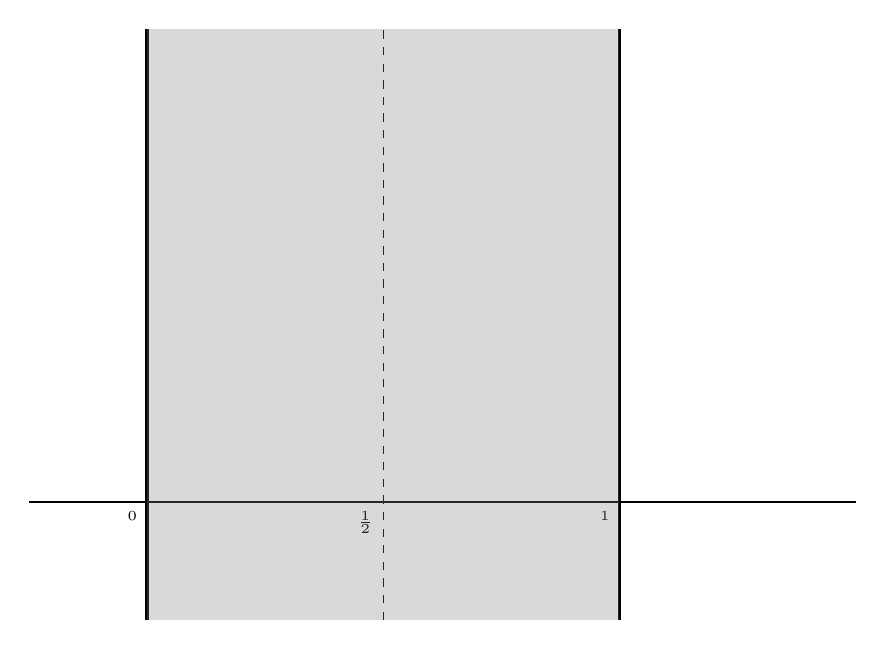
\begin{tikzpicture}[scale=3]
          \def\xmin{-0.5} \def\xmax{3}
          \def\ymin{-0.5} \def\ymax{2}
          \draw[thick] (\xmin,0) -- (\xmax,0);
          \draw[very thick] (0,\ymin) -- (0,\ymax);
          \draw[very thick] (2,\ymin) -- (2,\ymax);
          \draw[dashed] (1,\ymin) -- (1,\ymax);

          \node at (0,0) [below left] {\tiny{$0$}};
          \node at (1,0) [below left] {\tiny{$\frac{1}{2}$}};
          \node at (2,0) [below left] {\tiny{$1$}};

          \begin{scope}
            \path[clip] (0,\ymin) -- (0,\ymax) -- (2,\ymax) -- (2,\ymin) -- cycle;
            \fill[gray,opacity=0.3] (0,\ymin) rectangle (2,\ymax);
          \end{scope}
        \end{tikzpicture}
        \caption{The critical strip and critical line.}
        \label{fig:critical_strip}
      \end{figure}
  \section{The Riemann Zeta Function}\label{sec:The_Riemann_Zeta_Function}
    \subsection*{The Definition \& Euler Product of \texorpdfstring{$\z$}{\z}(s)}
      The \textbf{Riemann zeta function}\index{Riemann zeta function} or simply the \textbf{zeta function}\index{zeta function} $\z(s)$ is defined as an $L$-series:
      \[
        \z(s) = \sum_{n \ge 1}\frac{1}{n^{s}}.
      \]
      This is the prototypical example of a Dirichlet series as all the coefficients are $1$. Our main goal is to show that $\z(s)$ belongs to the Selberg class. As the coefficients are trivially polynomially bounded, $\z(s)$ is absolutely uniformly convergent on compacta for $\Re(s) > 1$. Also note that $\z(s)$ is necessiarly non-zero in this region. Determining the Euler product is also an easy matter. As the coefficients are obviously completely multiplicative, we have the degree $1$ Euler product
      \[
        \z(s) = \prod_{p}(1-p^{-s})^{-1},
      \]
      in this region as well. The local factor at $p$ is $(1-p^{-s})^{-1}$ with local root $1$. In particular, we have shown that the zeta function satisfies property (i) of the Selberg class and we package this into a theorem:

      \begin{theorem}
        For $\Re(s) > 1$,
        \[
          \z(s) = \prod_{p}(1-p^{-s})^{-1},
        \]
        is absolutely uniformly convergent on compacta with degree $1$ Euler product.
      \end{theorem}
    \subsection*{The Integral Representation of \texorpdfstring{$\z(s)$}{\z(s)}: Part I}
      Riemann's ingenious insight was to analytically continue $\z(s)$. By this, he sought to find a representation of $\z(s)$ defined on a larger region than $\Re(s) > 1$. This is the approach we will take, and the argument follows the same line of reasoning as that of Riemann. We consider the gamma function $\G\left(\frac{s}{2}\right)$:
      \[
        \G\left(\frac{s}{2}\right) = \int_{0}^{\infty}e^{-x}x^{\frac{s}{2}}\,\frac{dx}{x}.
      \]

      \begin{remark}
        We have chosen to express the gamma function in terms of the measure $\frac{dx}{x}$ instead of $dx$. This is a tactical change for two reasons. The first is that $\frac{dx}{x}$ is invariant under the change of variables $x \to Cx$ for any constant $C$. The second is that under the change of variables $x \to \frac{1}{x}$ we have $\frac{dx}{x} \to -\frac{dx}{x}$ but the bounds of integration are also flipped. So we may leave the measure invariant provided we dont flip the bounds of integration. These types of change of variables are essential in the study of $L$-functions which motivates the use of this measure.
      \end{remark}

      Performing the change of variables $x \to \pi n^{2}x$ for fixed $n \ge 1$ yields
      \begin{equation}\label{equ:gamma_integral_substitution}
        \G\left(\frac{s}{2}\right) = \pi^{\frac{s}{2}} n^{s}\int_{0}^{\infty}e^{-\pi n^{2}x}x^{\frac{s}{2}}\,\frac{dx}{x}.
      \end{equation}
      Dividing by $\pi^{\frac{s}{2}}n^{s}$ and summing over $n \ge 1$, we see that for $\Re(s) > 1$,
      \begin{align*}
        \pi^{-\frac{s}{2}}\G\left(\frac{s}{2}\right)\z(s) &= \sum_{n \ge 1}\int_{0}^{\infty}e^{-\pi n^{2}x}x^{\frac{s}{2}}\,\frac{dx}{x} \\
        &= \int_{0}^{\infty}\sum_{n \ge 1}e^{-\pi n^{2}x}x^{\frac{s}{2}}\,\frac{dx}{x} && \text{DCT} \\
        &= \int_{0}^{\infty}\w(x)x^{\frac{s}{2}}\,\frac{dx}{x},
      \end{align*}
      where we set
      \[
        \w(x) = \sum_{n \ge 1}e^{-\pi n^{2}x}.
      \]
      Therefore we have an integral representation
      \begin{equation}\label{equ:integral_representation_zeta_1}
        \z(s) = \frac{\pi^{\frac{s}{2}}}{\G\left(\frac{s}{2}\right)}\int_{0}^{\infty}\w(x)x^{\frac{s}{2}}\,\frac{dx}{x}.
      \end{equation}
      This was essentially Riemann's insight: rewrite the zeta function in terms of the Gamma function. Unfortunately, we cannot proceed until we understand $\w(x)$. So we will make a slight detour and come back to the integral representation after.
    \subsection*{Jacobi's Theta Function \texorpdfstring{$\vt(s)$}{\vt(s)}}
      \textbf{Jacobi's theta function}\index{Jacobi's theta function} $\vt(s)$ is defined for $\Re(s) > 0$ by
      \[
        \vt(s) = \sum_{n \in \Z}e^{-\pi n^{2}s} = 1+2\sum_{n \ge 1}e^{-\pi n^{2}s}.
      \]
      It is absolutely uniformly convergent on compacta in this region by the ratio test. It's relation to $\w(s)$ is the identity
      \begin{equation}\label{equ:omega_theta_relationship_for_zeta}
        \w(s) = \frac{\vt(s)-1}{2}.
      \end{equation}
      The essential fact about Jacobi's theta function we will need is the \textbf{transformation law for Jacobi's theta funtion}\index{transformation law for Jacobi's theta funtion} that was known to Riemann:

      \begin{theorem}[Transformation law for Jacobi's theta function]
        For $\Re(s) > 0$,
        \[
          \vt(s) = \frac{1}{\sqrt{s}}\vt\left(\frac{1}{s}\right).
        \]
      \end{theorem}
      \begin{proof}
        By the identity theorem it suffices to prove this on a set containg a limit point. We will prove this on the right-half of the real line, so take $s$ real with $s > 0$. Set $f(x) = e^{-\pi x^{2}s}$. Then $f(x)$ is a Schwarz function. We compute its Fourier transform:
        \[
          \hat{f}(t) = \int_{-\infty}^{\infty}f(x)e^{-2\pi itx}\,dx = \int_{-\infty}^{\infty}e^{-\pi x^{2}s}e^{-2\pi itx}\,dx = \int_{-\infty}^{\infty}e^{-\pi(x^{2}s+2itx)}\,dx.
        \]
        Making the change of variables $x \to \frac{x}{\sqrt{s}}$, the last integral above becomes
        \[
          \frac{1}{\sqrt{s}}\int_{-\infty}^{\infty}e^{-\pi\left(x^{2}+\frac{2itx}{\sqrt{s}}\right)}.
        \]
        Complete the square in the exponent by noticing
        \[
          -\pi\left(x^{2}+\frac{2itx}{\sqrt{s}}\right) = -\pi\left(\left(x+\frac{it}{\sqrt{s}}\right)^{2}+\frac{t^{2}}{s^{2}}\right).
        \]
        Taking exponentials, this implies that the previous integral is equal to
        \[
          \frac{e^{-\frac{\pi t^{2}}{s}}}{\sqrt{s}}\int_{-\infty}^{\infty}e^{-\pi\left(x+\frac{it}{\sqrt{s}}\right)^{2}}\,dx.
        \]
        We now treat this last integral as a complex integral. That is,
        \begin{equation}\label{transformation_law_for_Jacobi's_theta_function_1}
          \int_{-\infty}^{\infty}e^{-\pi\left(x+\frac{it}{\sqrt{s}}\right)^{2}}\,dx = \int_{\Im(z) = 0}e^{-\pi\left(z+\frac{it}{\sqrt{s}}\right)^{2}}\,dz = \int_{\Im(z) = \frac{t}{\sqrt{s}}}e^{-\pi z^{2}}\,dz,
        \end{equation}
        where in the last equality we have made the change of variables $z \to z-\frac{it}{\sqrt{s}}$. Now fix $T > 0$ and let $R_{T}$ be the positively oriented rectangle bounded by the lines $\Im(z) = 0$, $\Im(z) = \frac{t}{\sqrt{s}}$, $\Re(z) = -T$ and $\Re(z) = T$. Consider
        \[
          \lim_{T \to \infty}\int_{R_{T}}e^{-\pi z^{2}}\,dz.
        \]
        On the one hand, the residue theorem implies that the integral is the sum of a $2\pi i$ multiple of the residues in the rectangle $R_{T}$ and so the limit is the sum of a $2\pi i$ multiple of the residues in the strip bounded by $\Im(z) = 0$ and $\Im(z) = \frac{t}{\sqrt{s}}$. Since $e^{-\pi\left(z+\frac{it}{\sqrt{s}}\right)^{2}}$ is entire, this is zero. On the other hand, we can decompose the integral as
        \[
          \int_{\Im(z) = 0}e^{-\pi z^{2}}\,dz+\lim_{T \to \infty}\int_{0}^{\frac{t}{\sqrt{s}}}e^{-\pi(iz+T)^{2}}\,dz-\int_{\Im(z) = \frac{t}{\sqrt{s}}}e^{-\pi z^{2}}\,dz-\lim_{T \to \infty}\int_{0}^{\frac{t}{\sqrt{s}}}e^{-\pi(iz-T)^{2}}\,dz.
        \]
        Since $(iz \pm T)^{2} \ll_{z} T^{2}$, the integrands of the second and fourth terms decay to zero as $T \to \infty$. Hence the corresponding limits of integrals is zero. Putting these two remarks together shows
        \begin{equation}\label{transformation_law_for_Jacobi's_theta_function_2}
          \int_{\Im(z) = \frac{t}{\sqrt{s}}}e^{-\pi z^{2}}\,dz = \int_{\Im(z) = 0}e^{-\pi z^{2}}\,dz = \int_{-\infty}^{\infty}e^{-\pi x^{2}}\,dx.
        \end{equation}
        So back to the integral at hand, \cref{transformation_law_for_Jacobi's_theta_function_1,transformation_law_for_Jacobi's_theta_function_2} together imply
        \[
          \frac{e^{-\frac{\pi t^{2}}{s}}}{\sqrt{s}}\int_{-\infty}^{\infty}e^{-\pi\left(x+\frac{it}{\sqrt{s}}\right)^{2}}\,dx = \frac{e^{-\frac{\pi t^{2}}{s}}}{\sqrt{s}}\int_{-\infty}^{\infty}e^{-\pi x^{2}}\,dx = \frac{e^{-\frac{\pi t^{2}}{s}}}{\sqrt{s}},
        \]
        where the last equality follows because the last integral above is $1$ since it is the Gaussian integral (see \cref{append:Special_Integrals}). The Poisson summation formula and the identity theorem together finish the proof.
      \end{proof}

      Take note that the key ingredient in the proof was the Poisson summation formula. This is typical of a larger relaity when one needs to prove transformation laws. Also, the method of changing the line of integration from $\Im(z) = \frac{t}{\sqrt{s}}$ to $\Im(z) = 0$ works in a much more general setting and is a very useful analytic technique called \textbf{shifting the line of integration}\index{shifting the line of integration}:

      \begin{method}[Shifting the line of integration]
        Suppose we are given an integral
        \[
          \int_{\Re(z) = a}f(z)\,dz \quad \text{or} \quad \int_{\Im(z) = a}f(z)\,dz,
        \]
        and some real $b$ with $b < a$ in the first case and $b > a$ in the second case. Also suppose the following conditions hold corresponding to each case:
        \begin{enumerate}[label=(\roman*)]
          \item $f$ is meromorphic on a strip containing $\Re(z) = a,b$ or $\Im(z) = a,b$ respectively.
          \item $f$ is holomorphic about $\Re(z) = a,b$ or $\Im(z) = a,b$ respectively.
          \item $f(z) \to 0$ as $\Im(z) \to \infty$ or $f(z) \to 0$ as $\Re(z) \to \infty$ respectively.
        \end{enumerate}
        To collect these cases, let $(a)$ stand for the line $\Re(z) = a$ or $\Im(z) = a$ respectively with positive orientation. Then the line of integration $(a)$ can be shifted to the line of integration $(b)$ with the possible addition of residues. Take a rectangle $R_{T}$ given positive orientation and with its edges on $(a)$ and $(b)$ respectively and consider
        \[
          \lim_{T \to \infty}\int_{R_{T}}f(z)\,dz.
        \]
        On the one hand, the residue theorem implies the integral is a sum of a $2\pi i$ multiple of the residues $r_{i}$ in the rectangle $R_{T}$ and hence the limit is a sum of a $2\pi i$ multiple of the residues in the strip bounded by $(a)$ and $(b)$. Denote the corresponding set of poles inside this strip by $P$. On the other hand, the integral can be decomposed into a sum of four integrals along the edges of $R_{T}$ and by taking the limit the edges other than $(a)$ and $(b)$ will tend to zero because of the assumptions on $f$. The remaining two pieces is the difference between the integral along $(a)$ and $(b)$. So in total,
        \[
          \int_{(a)}f(z)\,dz = \int_{(b)}f(z)\,dz+2\pi i\sum_{\rho \in P}\Res_{z = \rho}f(z).
        \]
      \end{method}

      A particular application of interest is when the integral in question is real and over the entire real line, the integrand is entire as a complex function, and one is trying to shift the line of integration of the complexified integral to $\Im(z) = a$. In this case, shifting the line of integration amounts to making the change of variables $x \to x-ia$ without affecting the initial region of integration in the real integral. For example, in the proof of the transformation law for Jacobi's theta function this amounts to saying that the change of variables $x \to \frac{x}{\sqrt{s}}-\frac{it}{\sqrt{s}}$ is permitted without affecting the line of integration. We will appeal to this application often when proving transformation laws and one should become familiar with it. This completes our interest in Jacobi's theta function.
    \subsection*{The Integral Representation of \texorpdfstring{$\z(s)$}{\z(s)}: Part II}
      Returning to the zeta function, we split the integral in \cref{equ:integral_representation_zeta_1} into two pieces
      \begin{equation}\label{equ:symmetric_integral_zeta_split}
        \int_{0}^{\infty}\w(x)x^{\frac{s}{2}}\,\frac{dx}{x} = \int_{0}^{1}\w(x)x^{\frac{s}{2}}\,\frac{dx}{x}+\int_{1}^{\infty}\w(x)x^{\frac{s}{2}}\,\frac{dx}{x}.
      \end{equation}
      Since $\w(x)$ has exponential decay to zero as $x \to \infty$, the second piece is absolutely uniformly bounded on compacta for $\Re(s) > 1$ by \cref{met:decay_compacta_integral}. Hence it defines an analytic function there. The idea now is to rewrite the first piece in the same form and symmetrize the result as much as possible. We being by performing a change of variables $x \to \frac{1}{x}$ to the first piece to obtain
      \[
        \int_{1}^{\infty}\w\left(\frac{1}{x}\right)x^{-\frac{s}{2}}\,\frac{dx}{x}
      \]
      Now the transformation law for $\vt(x)$ and \cref{equ:omega_theta_relationship_for_zeta} together imply
      \begin{equation}\label{equ:piece_one_zeta_1}
        \w\left(\frac{1}{x}\right) = \frac{\vt\left(\frac{1}{x}\right)-1}{2} = \frac{\sqrt{x}\vt(x)-1}{2} = \frac{\sqrt{x}(2\w(x)+1)-1}{2} = \sqrt{x}\w(x)+\frac{\sqrt{x}}{2}-\frac{1}{2}.
      \end{equation}
      \cref{equ:piece_one_zeta_1} gives the first equality in the following chain:
      \begin{align*}
        \int_{1}^{\infty}\w\left(\frac{1}{x}\right)x^{-\frac{s}{2}}\,\frac{dx}{x} &= \int_{1}^{\infty}\left(\sqrt{x}\w(x)+\frac{\sqrt{x}}{2}-\frac{1}{2}\right)x^{-\frac{s}{2}}\,\frac{dx}{x} \\
        &= \int_{1}^{\infty}\w(x)x^{\frac{1-s}{2}}\,\frac{dx}{x}+\int_{1}^{\infty}\frac{x^{\frac{1-s}{2}}}{2}\,\frac{dx}{x}-\int_{1}^{\infty}\frac{x^{-\frac{s}{2}}}{2}\,\frac{dx}{x} \\
        &= \int_{1}^{\infty}\w(x)x^{\frac{1-s}{2}}\,\frac{dx}{x}+\frac{1}{1-s}-\frac{1}{s} \\
        &= \int_{1}^{\infty}\w(x)x^{\frac{1-s}{2}}\,\frac{dx}{x}-\frac{1}{s(1-s)}.
      \end{align*}
      Substituting this result back into \cref{equ:symmetric_integral_zeta_split} with \cref{equ:integral_representation_zeta_1} yields the following result:

      \begin{theorem}
        For $\Re(s) > 1$,
        \[
          \z(s) = \frac{\pi^{\frac{s}{2}}}{\G\left(\frac{s}{2}\right)}\left[-\frac{1}{s(1-s)}+\int_{1}^{\infty}\w(x)x^{\frac{1-s}{2}}\,\frac{dx}{x}+\int_{1}^{\infty}\w(x)x^{\frac{s}{2}}\,\frac{dx}{x}\right].
        \]
      \end{theorem}

      This integral representation will give analytic continuation. To see this, first observe that we know everything outside the backets is entire. Everything inside the brackets except for the first integral is analytic for $\Re(s) > 1$. Thus the first integral must be analytic in this region too. Since the two integrals are interchanged as $s \to 1-s$ and the rational term $-\frac{1}{s(1-s)}$ is invariant, the right-hand side is analytic for $\Re(s) < 0$. This gives the analytic continuation of $\z(s)$ to the region
      \[
        \left\{s \in \C:\left|\Re(s)-\frac{1}{2}\right| > \frac{1}{2}\right\}.
      \]
    \subsection*{The Functional Equation, Critical Strip \& Residue of \texorpdfstring{$\z(s)$}{\z(s)}}
      An immediate consequence of the symmetry of the integral representation is the functional equation:
      \[
        \frac{\G\left(\frac{s}{2}\right)}{\pi^{\frac{s}{2}}}\z(s) = \frac{\G\left(\frac{1-s}{2}\right)}{\pi^{\frac{1-s}{2}}}\z(1-s).
      \]
      We identify the gamma factor as
      \[
        \g(s,\z) = \pi^{-\frac{s}{2}}\G\left(\frac{s}{2}\right),
      \]
      with $\k = \frac{s}{2}$ the only local parameter at infinity. Clearly it satisfies the required bounds. The conductor is $q(\z) = 1$ so no primes ramify. The completed zeta function is
      \[
        \L(s,\z) = \pi^{-\frac{s}{2}}\G\left(\frac{s}{2}\right)\z(s),
      \]
      with functional equation
      \[
        \L(s,\z) = \L(1-s,\z).
      \]
      This is the functional equation of $\z(s)$ and in this case is just a reformulation of the previous functional equation. From it we find that the root number is $\e(\z) = 1$ and that $\z$ is self-dual. Altogether, we have shown that $\z$ satisfies properties (ii)-(iv) of the Selberg class.

      Having obtained the funtional equation, we now use the integral representation to obtain meromorphic continuation of $\z(s)$ inside the critical strip. From the integral representation, we have
      \begin{equation}\label{equ:integral_representation_zeta_2}
        \z(s) = \frac{1}{\g(s,\z)}\left[-\frac{1}{s(1-s)}+\int_{1}^{\infty}\w(x)x^{\frac{1-s}{2}}\,\frac{dx}{x}+\int_{1}^{\infty}\w(x)x^{\frac{s}{2}}\,\frac{dx}{x}\right].
      \end{equation}
      To get continuation inside of the critical strip, we argue that the two integrals are absolutely uniformly bounded on compacta for $|\Re(s)-\frac{1}{2}| \le \frac{1}{2}$. This follows by \cref{met:decay_compacta_integral} (we could have gotten this continuation earlier but we didn't need it until now). If we assume $s \neq 0,1$, then the analytic continuation to the inside of the critical strip follows since the fractional term $\frac{1}{s(1-s)}$ is holomorphic there. The cases $s = 0,1$ require separate inspection. When $s = 0$, $\g(s,\z)$ has a simple pole coming from the gamma factor, and therefore its reciprocal has a simple zero. This cancels the corresponding simple pole of $\frac{1}{s(1-s)}$ so that $\z(s)$ has a removable singularity and thus is holomorphic at $s = 0$. At $s = 1$, $\g(s,\z)$ is non-zero, and so $\z(s)$ has a simple pole. Therefore $\z(s)$ has meromorphic continuation to all of $\C$ with a simple pole at $s = 1$.

      We can now show that the order of $\z(s)$ is $1$ and conclude that it satisfies property (v) of the Selberg class, and is therefore an $L$-function belonging to the Selberg class. As there is only a simple pole at $s = 1$, multiply by $(s-1)$ to clear the polar divisor. Now the integral in the integral representation is absolutely bounded, so computing the order amounts to estimating the gamma factor. Since the reciprocal of the gamma function is of order $1$ and $\Re(s)$ is bounded, we have
      \begin{equation}\label{equ:zeta_function_gamma_factor_order_1}
        \frac{1}{\g(s,\z)} \ll_{\e} e^{|s|^{1+\e}},
      \end{equation}
      for any $\e > 0$. So the reciprocal of the gamma factor is of the same order. Then \cref{equ:zeta_function_gamma_factor_order_1,equ:integral_representation_zeta_2} together imply
      \[
        (s-1)\z(s) \ll_{\e} e^{|s|^{1+\e}}.
      \]
      So $(s-1)\z(s)$ is of order $1$, and thus $\z(s)$ is as well after removing the polar factor. Having shown the analytic continuation of $\z(s)$, and verified that it belongs to the Selberg class, there is only one thing left to do. This is to compute the residue of $\z(s)$ at $s = 1$:

      \begin{proposition}\label{prop:zeta_residue}
        \[
          \Res_{s = 1}\z(s) = 1.
        \]
      \end{proposition}
      \begin{proof}
        The only term in the integral representation of $\z(s)$ contributing to the pole is $-\frac{1}{\g(s,\z)}\frac{1}{s(1-s)}$. Observe
        \[
          \lim_{s \to 1}\frac{1}{\g(s,\z)} = \lim_{s \to 1}\frac{\pi^{\frac{s}{2}}}{\G\left(\frac{s}{2}\right)} = 1,
        \]
        because $\G\left(\frac{1}{2}\right) = \sqrt{\pi}$. Therefore
        \[
          \Res_{s = 1}\z(s) = \Res_{s = 1}-\frac{1}{\g(s,\z)}\frac{1}{s(1-s)} = \Res_{s = 1}-\frac{1}{s(1-s)} = \lim_{s \to 1}-\frac{(s-1)}{s(1-s)} = 1.
        \]
      \end{proof}

      We summarize all of our work into the following theorem:

      \begin{theorem}
        $\z(s)$ is a Selberg class $L$-function. It admits meromorphic continuation to $\C$ via the integral representation
        \[
          \z(s) = \frac{\pi^{\frac{s}{2}}}{\G\left(\frac{s}{2}\right)}\left[-\frac{1}{s(1-s)}+\int_{1}^{\infty}\w(x)x^{\frac{1-s}{2}}\,\frac{dx}{x}+\int_{1}^{\infty}\w(x)x^{\frac{s}{2}}\,\frac{dx}{x}\right],
        \]
        with functional equation
        \[
          \pi^{-\frac{s}{2}}\G\left(\frac{s}{2}\right)\z(s) = \L(s,\z) = \L(1-s,\z),
        \]
        and there is a simple pole at $s = 1$ of residue $1$.
      \end{theorem}

      Lastly, we note that by virtue of the functional equation we can also compute $\z(0)$ as well. Indeed, since $\Res_{s = 1}\z(s) = 1$, we have
        \[
          \lim_{s \to 1}(s-1)\L(s,\z) = \Res_{s = 1}\z(s)\lim_{s \to 1}\pi^{-\frac{s}{2}}\G\left(\frac{s}{2}\right) = 1.
        \]
        In other words, $\L(s,\z)$ has a simple pole at $s = 1$ with residue $1$ too. Since the completed zeta function is completely symmetric as $s \to 1-s$, it has a simple pole at $s = 0$ with residue $1$. Hence
        \[
          1 = \lim_{s \to 1}(s-1)\L(1-s,\z) = \Res_{s = 1}\G\left(\frac{1-s}{2}\right)\lim_{s \to 1}\pi^{-\frac{1-s}{2}}\z(1-s) = -2\z(0),
        \]
        because $\Res_{s = 0}\G(s) = 1$. Therefore $\z(0) = -\frac{1}{2}$.
  \section{Dirichlet \texorpdfstring{$L$}{L}-functions}
    \subsection*{The Definition \& Euler Product of \texorpdfstring{$L(s,\chi)$}{L(s,\chi)}}
      To every Dirichlet character $\chi$ there is an associated $L$-function. Throughout we will let $m$ denote the modulus and $q$ the conductor of $\chi$ respectively. The \textbf{Dirichlet $L$-function}\index{Dirichlet $L$-function} $L(s,\chi)$ attached to the Dirichlet character $\chi$ is defined as an $L$-series:
      \[
        L(s,\chi) = \sum_{n \ge 1}\frac{\chi(n)}{n^{s}}.
      \]
      Since $\chi(n) = 0$ if $(n,m) > 1$, the above sum can be restricted to all integers relatively prime to $m$. We first obtain convergence in a half-plane. As $|\chi(n)| \ll 1$, $L(s,\chi)$ is absolutely uniformly convergent on compacta for $\Re(s) > 1$ just as is the case for $\z(s)$. Because $\chi$ is completely multiplicative we also have the degree $1$ Euler product,
      \[
        L(s,\chi) = \prod_{p}(1-\chi(p)p^{-s})^{-1} = \prod_{p \nmid m}(1-\chi(p)p^{-s})^{-1},
      \]
      in this region as well. The last equality holds because if $p \mid m$ we have $\chi(p) = 0$. So for $p \mid m$, the local factor at $p$ is $1$ with local root $0$. For $p \nmid m$ the local factor at $p$ is $(1-\chi(p)p^{-s})^{-1}$ with local root $\chi(p)$. Now if $\chi$ is induced by $\wtilde{\chi}$, then $\chi(p) = \wtilde{\chi}(p)$ if $p \nmid q$ and $\chi(p) = 0$ if $p \mid m$ so that
      \begin{equation}\label{equ:non-primitive_primitive_Dirichlet_L-series_relation}
        L(s,\chi) = \prod_{p \nmid m}(1-\wtilde{\chi}(p)p^{-s})^{-1} = \prod_{p}(1-\wtilde{\chi}(p)p^{-s})^{-1}\prod_{p \mid m}(1-\wtilde{\chi}(p)p^{-s}) = L(s,\wtilde{\chi})\prod_{p \mid m}(1-\wtilde{\chi}(p)p^{-s}).
      \end{equation}
      Therefore $L(s,\chi)$ belongs to the Selberg class if and only if $L(s,\wtilde{\chi})$ does. So we may assume $\chi$ is primitive. We may assume further that $q > 1$ because if not $\chi$ is principal which means $\wtilde{\chi}$ is trivial so that $L(s,\wtilde{\chi}) = \z(s)$, and this $L$-function already belongs to the Selberg class. Our main goal is now to show that $L(s,\chi)$ is a Selberg class $L$-function when $\chi$ is primitive and $q > 1$. We have already shown that $L(s,\chi)$ satisfies property (i) of the Selberg class and we package this into a theorem:

      \begin{theorem}
        Let $\chi$ be a primitive Dirichlet character with conductor $q > 1$. For $\Re(s) > 1$,
        \[
          L(s,\chi) = \prod_{p}(1-\chi(p)p^{-s})^{-1} = \prod_{p \nmid q}(1-\chi(p)p^{-s})^{-1},
        \]
        is absolutely uniformly convergent on compacta with degree $1$ Euler product.
      \end{theorem}
    \subsection*{The Integral Representation of \texorpdfstring{$L(s,\chi)$}{L(s,\chi)}: Part I}
      To find the integral representation for $L(s,\chi)$, we argue in a manner similar to $\z(s)$. However, the following will depend if $\chi$ is even or odd, so to handle both cases simultaneously let $\mf{a} = 0,1$ according to whether $\chi$ is even or odd. In particular, $\chi(-1) = (-1)^{\mf{a}}$. Note that $\mf{a}$ takes the same value for both $\chi$ and $\cchi$. Making the substitution $s \to s+\mf{a}$ in \cref{equ:gamma_integral_substitution} and multiplying by $\chi(n)$ yields
      \[
        \chi(n)\G\left(\frac{s+\mf{a}}{2}\right) = \pi^{\frac{s+\mf{a}}{2}} n^{s}\int_{0}^{\infty}\chi(n)n^{\mf{a}}e^{-\pi n^{2}x}x^{\frac{s+\mf{a}}{2}}\,\frac{dx}{x},
      \]
      after moving the $n^{\mf{a}}$ on the inside of the integral. Dividing by $\pi^{\frac{s+\mf{a}}{2}}n^{s}$ and summing over $n \ge 1$, we see that for $\Re(s) > 1$,
      \begin{align*}
        \pi^{-\frac{s+\mf{a}}{2}}\G\left(\frac{s+\mf{a}}{2}\right)L(s,\chi) &= \sum_{n \ge 1}\int_{0}^{\infty}\chi(n)n^{\mf{a}}e^{-\pi n^{2}x}x^{\frac{s+\mf{a}}{2}}\,\frac{dx}{x} \\
        &= \int_{0}^{\infty}\sum_{n \ge 1}\chi(n)n^{\mf{a}}e^{-\pi n^{2}x}x^{\frac{s+\mf{a}}{2}}\,\frac{dx}{x} && \text{DCT} \\
        &= \int_{0}^{\infty}\w_{\chi}(x)x^{\frac{s+\mf{a}}{2}}\,\frac{dx}{x},
      \end{align*}
      where we set
      \[
        \w_{\chi}(x) = \sum_{n \ge 1}\chi(n)n^{\mf{a}}e^{-\pi n^{2}x}.
      \]
      Therefore we have an integral representation
      \begin{equation}\label{equ:integral_representation_Dirichlet_L-functions_1}
        L(s,\chi) = \frac{\pi^{\frac{s+\mf{a}}{2}}}{\G\left(\frac{s+\mf{a}}{2}\right)}\int_{0}^{\infty}\w_{\chi}(x)x^{\frac{s+\mf{a}}{2}}\,\frac{dx}{x},
      \end{equation}
      and just like $\z(s)$ we need to find a transformation law for $\w_{\chi}(x)$ before we can proceed.
    \subsection*{The Dirichlet Theta Function \texorpdfstring{$\vt_{\chi}(s)$}{\vt_{\chi}(s)}}
      The \textbf{Dirichlet theta function}\index{Dirichlet theta function} $\vt_{\chi}(s)$, attached to the character $\chi$, is defined for $\Re(s) > 0$ by
      \[
        \vt_{\chi}(s) = \sum_{n \in \Z}\chi(n)n^{\mf{a}}e^{-\pi n^{2}s} = 2\sum_{n \ge 1}\chi(n)n^{\mf{a}}e^{-\pi n^{2}s}.
      \]
      It is absolutely uniformly convergent on compacta in this region by the ratio test. Notice that the term corresponding to $n = 0$ vanishes because $\chi(0) = 0$, and $\chi(n)n^{\mf{a}} = \chi(-n)(-n)^{\mf{a}}$ so that the $n$-th and $(-n)$-th terms agree. Therefore the relationship between the twisted theta function and $\w_{\chi}(s)$ is
      \begin{equation}\label{equ:twisted_omega_theta_relationship_for_Dirichlet_L-functions}
        \w_{\chi}(s) = \frac{\vt_{\chi}(s)}{2}.
      \end{equation}

      \begin{remark}
        \cref{equ:twisted_omega_theta_relationship_for_Dirichlet_L-functions} is a slightly less complex relationship that \cref{equ:omega_theta_relationship_for_zeta}. This is because assuming $q > 1$ means $\chi(0) = 0$.
      \end{remark}

      The essential fact about the twisted theta function we will need is the following transformation law similar to the transformation law for Jacobi's theta function:

      \begin{theorem}
        Let $\chi$ be a primitive Dirichlet character with conductor $q > 1$. For $\Re(s) > 0$,
        \[
          \vt_{\chi}(s) = \frac{\e_{\chi}}{i^{\mf{a}}(qs)^{\frac{1}{2}+\mf{a}}}\vt_{\cchi}\left(\frac{1}{q^{2}s}\right).
        \]
      \end{theorem}
      \begin{proof}
        By the identity theorem it suffices to prove this on a set containg a limit point. We will prove this on the right-half of the real line, so take $s$ real with $s > 0$. Since $\chi$ is $q$-periodic, we can write
        \[
          \vt_{\chi}(s) = \sum_{a \tmod{q}}\chi(a)\sum_{m \in \Z}(mq+a)^{\mf{a}}e^{-\pi(mq+a)^{2}s}.
        \]
        Set $f(x) = (xq+a)^{\mf{a}}e^{-\pi(xq+a)^{2}s}$. Then $f(x)$ is a Schwarz function. We compute its Fourier transform:
        \[
          \hat{f}(t) = \int_{-\infty}^{\infty}f(x)e^{-2\pi itx}\,dx = \int_{-\infty}^{\infty}(xq+a)^{\mf{a}}e^{-\pi(xq+a)^{2}s}e^{-2\pi itx}\,dx = \int_{-\infty}^{\infty}(xq+a)^{\mf{a}}e^{-\pi((xq+a)^{2}s+2itx)}\,dx.
        \]
        By performing the change of variables $x \to \frac{x}{q\sqrt{s}}-\frac{a}{q}$, the last integral above becomes
        \[
          \frac{e^{\frac{2\pi iat}{q}}}{qs^{\frac{1+\mf{a}}{2}}}\int_{-\infty}^{\infty}x^{\mf{a}}e^{-\pi\left(x^{2}+\frac{2itx}{q\sqrt{s}}\right)}\,dx.
        \]
        Complete the square in the exponent by observing
        \[
          -\pi\left(x^{2}+\frac{2itx}{q\sqrt{s}}\right) = -\pi\left(\left(x+\frac{it}{q\sqrt{s}}\right)^{2}+\frac{t^{2}}{q^{2}s}\right).
        \]
        Taking exponentials, this implies that the previous integral is equal to
        \[
          \frac{e^{\frac{2\pi iat}{q}}e^{-\frac{\pi t^{2}}{q^{2}s}}}{qs^{\frac{1+\mf{a}}{2}}}\int_{-\infty}^{\infty}x^{\mf{a}}e^{-\pi\left(x+\frac{it}{q\sqrt{s}}\right)^{2}}\,dx.
        \]
        The change of variables $x \to x-\frac{it}{q\sqrt{s}}$ is permitted without affecting the line of integration by viewing the integral as a complex integral, noting that the integrand is entire as a complex function, and shifting the line of integration. This gives
        \[
          \frac{e^{\frac{2\pi iat}{q}}e^{-\frac{\pi t^{2}}{q^{2}s}}}{qs^{\frac{1+\mf{a}}{2}}}\int_{-\infty}^{\infty}\left(x-\frac{it}{q\sqrt{s}}\right)^{\mf{a}}e^{-\pi x^{2}}\,dx = \frac{e^{\frac{2\pi iat}{q}}e^{-\frac{\pi t^{2}}{q^{2}s}}}{qs^{\frac{1+\mf{a}}{2}}}\int_{-\infty}^{\infty}\left(x+\frac{t}{iq\sqrt{s}}\right)^{\mf{a}}e^{-\pi x^{2}}\,dx.
        \]
        If $\mf{a} = 0$, we obtain
        \begin{equation}\label{transformation_law_for_twisted_Jacobi's_theta_function_1}
          \frac{e^{\frac{2\pi iat}{q}}e^{-\frac{\pi t^{2}}{q^{2}s}}}{qs^{\frac{1+\mf{a}}{2}}}\int_{-\infty}^{\infty}e^{-\pi x^{2}}\,dx = \frac{e^{\frac{2\pi iat}{q}}e^{-\frac{\pi t^{2}}{q^{2}s}}}{qs^{\frac{1+\mf{a}}{2}}},
        \end{equation}
        where the equality holds because the integral is $1$ since it is the Gaussian integral (see \cref{append:Special_Integrals}). If $\mf{a} = 1$, then by direct computation
        \[
          \int_{-\infty}^{\infty}xe^{-\pi x^{2}}\,dx = -\frac{1}{2\pi}e^{-\pi x^{2}}\bigg|_{-\infty}^{\infty} = 0,
        \]
        and thus
        \begin{equation}\label{transformation_law_for_twisted_Jacobi's_theta_function_2}
          \frac{e^{\frac{2\pi iat}{q}}e^{-\frac{\pi t^{2}}{q^{2}s}}}{qs^{\frac{1+\mf{a}}{2}}}\int_{-\infty}^{\infty}\left(\frac{t}{iq\sqrt{s}}\right)e^{-\pi x^{2}}\,dx = \frac{e^{\frac{2\pi iat}{q}}e^{-\frac{\pi t^{2}}{q^{2}s}}}{qs^{\frac{1+\mf{a}}{2}}}\left(\frac{t}{iq\sqrt{s}}\right)\int_{-\infty}^{\infty}e^{-\pi x^{2}}\,dx = \frac{e^{\frac{2\pi iat}{q}}e^{-\frac{\pi t^{2}}{q^{2}s}}}{qs^{\frac{1+\mf{a}}{2}}}\left(\frac{t}{iq\sqrt{s}}\right),
        \end{equation}
        where the last equality follows because the last integral is the Gaussian integral again. Since $\left(\frac{t}{iq\sqrt{s}}\right)^{\mf{a}} = 1$ if $\mf{a} = 0$, we can compactly express the right-hand sides of \cref{transformation_law_for_twisted_Jacobi's_theta_function_1,transformation_law_for_twisted_Jacobi's_theta_function_2} in the form
        \[
          \frac{e^{\frac{2\pi iat}{q}}e^{-\frac{\pi t^{2}}{q^{2}s}}}{qs^{\frac{1+\mf{a}}{2}}}\left(\frac{t}{iq\sqrt{s}}\right)^{\mf{a}}.
        \]
        The Poisson summation formula then implies
        \begin{align*}
          \vt_{\chi}(s) &= \sum_{a \tmod{q}}\chi(a)\sum_{t \in \Z}\frac{e^{\frac{2\pi iat}{q}}e^{-\frac{\pi t^{2}}{q^{2}s}}}{qs^{\frac{1+\mf{a}}{2}}}\left(\frac{t}{iq\sqrt{s}}\right)^{\mf{a}} \\
          &= \frac{1}{i^{\mf{a}}q^{1+\mf{a}}s^{\frac{1}{2}+\mf{a}}}\sum_{a \tmod{q}}\chi(a)\sum_{t \in \Z}t^{\mf{a}}e^{\frac{2\pi i at}{q}}e^{-\frac{\pi t^{2}}{q^{2}s}} \\
          &= \frac{1}{i^{\mf{a}}q^{1+\mf{a}}s^{\frac{1}{2}+\mf{a}}}\sum_{t \in \Z}t^{\mf{a}}e^{-\frac{\pi t^{2}}{q^{2}s}}\sum_{a \tmod{q}}\chi(a)e^{\frac{2\pi i at}{q}} \\
          &= \frac{1}{i^{\mf{a}}q^{1+\mf{a}}s^{\frac{1}{2}+\mf{a}}}\sum_{t \in \Z}t^{\mf{a}}e^{-\frac{\pi t^{2}}{q^{2}s}}\tau(t,\chi) && \text{definition of $\tau(t,\chi)$},
        \end{align*}
        and this holds for all $\Re(s) > 0$ by the identity theorem. Since $\chi$ is primitive, $\tau(t,\chi) = 0$ if $(t,q) > 1$ and otherwise $\tau(t,\chi) = \cchi(t)\tau(1,\chi)$ (see \cref{prop:Gauss_sum_reduction}). Therefore we have
        \[
          \frac{1}{i^{\mf{a}}q^{1+\mf{a}}s^{\frac{1}{2}+\mf{a}}}\sum_{t \in \Z}t^{\mf{a}}e^{-\frac{\pi t^{2}}{q^{2}s}}\tau(t,\chi) = \frac{\tau(1,\chi)}{i^{\mf{a}}q^{1+\mf{a}}s^{\frac{1}{2}+\mf{a}}}\sum_{t \in \Z}\cchi(t)t^{\mf{a}}e^{-\frac{\pi t^{2}}{q^{2}s}} = \frac{\tau(1,\chi)}{i^{\mf{a}}q^{1+\mf{a}}s^{\frac{1}{2}+\mf{a}}}\vt_{\cchi}\left(\frac{1}{q^{2}s}\right).
        \]
        Recalling that $\e_{\chi} = \frac{\tau(1,\chi)}{\sqrt{q}}$, we conclude
        \[
          \vt_{\chi}(s) = \frac{\e_{\chi}}{i^{\mf{a}}(qs)^{\frac{1}{2}+\mf{a}}}\vt_{\cchi}\left(\frac{1}{q^{2}s}\right).
        \]
      \end{proof}
      The most striking property about this transformation law is that it relates $\vt_{\chi}(s)$ and $\vt_{\cchi}(s)$. Regardless, we can now exploit it to analytically continue $L(s,\chi)$.
    \subsection*{The Integral Representation of \texorpdfstring{$L(s,\chi)$}{L(s,\chi)}: Part II}
      Returning to $L(s,\chi)$, split the integral in \cref{equ:integral_representation_Dirichlet_L-functions_1} into two pieces
      \begin{equation}\label{equ:symmetric_integral_Dirichlet_L-functions_split}
        \int_{0}^{\infty}\w_{\chi}(x)x^{\frac{s+\mf{a}}{2}}\,\frac{dx}{x} = \int_{0}^{\frac{1}{q}}\w_{\chi}(x)x^{\frac{s+\mf{a}}{2}}\,\frac{dx}{x}+\int_{\frac{1}{q}}^{\infty}\w_{\chi}(x)x^{\frac{s+\mf{a}}{2}}\,\frac{dx}{x}.
      \end{equation}
      Since $\w_{\chi}(x)$ has exponential decay to zero as $x \to \infty$, the second piece is absolutely uniformly bounded on compacta for $\Re(s) > 1$ by \cref{met:decay_compacta_integral}. Hence it defines an analytic function there. We now rewrite the first piece in the same form and symmetrize the result as much as possible. Start by performing a change of variables $x \to \frac{1}{q^{2}x}$ to the first piece to obtain
      \[
        q^{-(s+\mf{a})}\int_{\frac{1}{q}}^{\infty}\w_{\chi}\left(\frac{1}{q^{2}x}\right)x^{-\frac{s+\mf{a}}{2}}\,\frac{dx}{x}.
      \]
      Now the transformation law for $\vt_{\chi}(x)$ and \cref{equ:twisted_omega_theta_relationship_for_Dirichlet_L-functions} together imply
      \begin{equation}\label{equ:piece_one_Dirichlet_1}
        \begin{aligned}
          \w_{\chi}\left(\frac{1}{q^{2}x}\right) &= \frac{\vt_{\chi}\left(\frac{1}{q^{2}x}\right)}{2} \\
          &= \frac{i^{\mf{a}}(qx)^{\frac{1}{2}+\mf{a}}}{\e_{\cchi}}\frac{\vt_{\cchi}(x)}{2} \\
          &= \e_{\chi}(-i)^{\mf{a}}(qx)^{\frac{1}{2}+\mf{a}}\frac{\vt_{\cchi}(x)}{2} && \text{\cref{prop:epsilon_factor_relationship} and $\chi(-1) = (-1)^{\mf{a}}$} \\
          &= \frac{\e_{\chi}(qx)^{\frac{1}{2}+\mf{a}}}{i^{\mf{a}}}\frac{\vt_{\cchi}(x)}{2} \\
          &= \frac{\e_{\chi}(qx)^{\frac{1}{2}+\mf{a}}}{i^{\mf{a}}}\w_{\cchi}(x).
        \end{aligned}
      \end{equation}
      \cref{equ:piece_one_Dirichlet_1} gives the first equality in the following chain:
      \begin{align*}
        q^{-(s+\mf{a})}\int_{\frac{1}{q}}^{\infty}\w_{\chi}\left(\frac{1}{q^{2}x}\right)x^{-\frac{s+\mf{a}}{2}}\,\frac{dx}{x} &= q^{-(s+\mf{a})}\int_{\frac{1}{q}}^{\infty}\left(\frac{\e_{\chi}(qx)^{\frac{1}{2}+\mf{a}}}{i^{\mf{a}}}\w_{\cchi}(x)\right)x^{-\frac{s+\mf{a}}{2}}\,\frac{dx}{x} \\
        &= \frac{\e_{\chi}}{i^{\mf{a}}}q^{\frac{1}{2}-s}\int_{\frac{1}{q}}^{\infty}\w_{\cchi}(x)x^{\frac{(1-s)+\mf{a}}{2}}\,\frac{dx}{x}.
      \end{align*}
      Substituting this last expression back into \cref{equ:symmetric_integral_Dirichlet_L-functions_split} with \cref{equ:integral_representation_Dirichlet_L-functions_1} gives the following result:
      \begin{theorem}
        Let $\chi$ be a primitive Dirichlet character with conductor $q > 1$. For $\Re(s) > 1$,
        \[
          L(s,\chi) = \frac{\pi^{\frac{s+\mf{a}}{2}}}{\G\left(\frac{s+\mf{a}}{2}\right)}\left[\frac{\e_{\chi}}{i^{\mf{a}}}q^{\frac{1}{2}-s}\int_{\frac{1}{q}}^{\infty}\w_{\cchi}(x)x^{\frac{(1-s)+\mf{a}}{2}}\,\frac{dx}{x}+\int_{\frac{1}{q}}^{\infty}\w_{\chi}(x)x^{\frac{s+\mf{a}}{2}}\,\frac{dx}{x}\right].
        \]
      \end{theorem}

      This integral representation will give analytic continuation. Indeed, we know everything outside the brackets is entire and the latter of the two integrals inside the brackets is analytic for $\Re(s) > 1$. Thus the first integral inside the brackets must be analytic in this region too. Since the two integrals are interchanged as $s \to 1-s$, save for the term $\frac{\e_{\chi}}{i^{\mf{a}}}q^{\frac{1}{2}-s}$, the right-hand side is analytic for $\Re(s) < 0$. This gives the analytic continuation of $L(s,\chi)$ to the region
      \[
        \left\{s \in \C:\left|\Re(s)-\frac{1}{2}\right| > \frac{1}{2}\right\}.
      \]
    \subsection*{The Functional Equation \& Critical Strip of \texorpdfstring{$L(s,\chi)$}{L(s,\chi)}}
      An immediate consequence of the symmetry of the integral representation is the functional equation:
      \[
        q^{\frac{s}{2}}\frac{\G\left(\frac{s+\mf{a}}{2}\right)}{\pi^{\frac{s+\mf{a}}{2}}}L(s,\chi) = \frac{\e_{\chi}}{i^{\mf{a}}}q^{\frac{1-s}{2}}\frac{\G\left(\frac{(1-s)+\mf{a}}{2}\right)}{\pi^{\frac{(1-s)+\mf{a}}{2}}}L(1-s,\cchi).
      \]
      We identify the gamma factor as
      \[
        \g(s,\chi) = \pi^{-\frac{s+\mf{a}}{2}}\G\left(\frac{s+\mf{a}}{2}\right),
      \]
      with $\k = \frac{s+\mf{a}}{2}$ the only local parameter at infinity. Clearly it satisfies the required bounds. The conductor is $q(\chi) = q$ and if $p$ is an unramified prime then the local root is $\chi(p) \neq 0$. The completed $L$-function is
      \[
        \L(s,\chi) = q^{\frac{s}{2}}\pi^{-\frac{s+\mf{a}}{2}}\G\left(\frac{s+\mf{a}}{2}\right)L(s,\chi),
      \]
      with functional equation
      \[
        \L(s,\chi) = \frac{\e_{\chi}}{i^{\mf{a}}}\L(1-s,\cchi).
      \]
      From it we see that the root number is $\e(\chi) = \frac{\e_{\chi}}{i^{\mf{a}}}$ and that $L(s,\chi)$ has dual $L(s,\cchi)$. In total, $L(s,\chi)$ satisfies properties (ii)-(iv) of the Selberg class.

      We now analytically continue $L(s,\chi)$ inside the critical strip and therefore to all of $\C$. From the integral representation, we have
      \begin{equation}\label{equ:integral_representation_Dirichlet_L-functions_2}
        L(s,\chi) = \frac{1}{\g(s,\chi)}\left[\frac{\e_{\chi}}{i^{\mf{a}}}q^{\frac{1}{2}-s}\int_{\frac{1}{q}}^{\infty}\w_{\cchi}(x)x^{\frac{(1-s)+\mf{a}}{2}}\,\frac{dx}{x}+\int_{\frac{1}{q}}^{\infty}\w_{\chi}(x)x^{\frac{s+\mf{a}}{2}}\,\frac{dx}{x}\right].
      \end{equation}
      To get continuation inside the critical strip it suffices that the two integrals are absolutely uniformly bounded on compacta for $|\Re(s)-\frac{1}{2}| \le \frac{1}{2}$. This follows by \cref{met:decay_compacta_integral} (we could have deduced this continuation earlier but we didn't need it until now) and thus gives analytic continuation to the critical strip and hence to all of $\C$. In particular, we have shown that $L(s,\chi)$ has no poles.

      All we are left to show is that $L(s,\chi)$ is of order $1$ to conclude that it satisfies property (v) of the Selberg class and therefore is an $L$-function belonging to the Selberg class. Since $L(s,\chi)$ has no poles, we do not need to clear any polar divisors. As the integral in the representation is absolutely bounded, computing the order amounts to estimating the gamma factor. Since the reciprocal of the gamma function is of order $1$ and $\Re(s)$ is bounded, we have
      \begin{equation}\label{equ:Dirichlet_L-functions_factor_order_1}
        \frac{1}{\g(s,\chi)} \ll_{\e} e^{|s|^{1+\e}},
      \end{equation}
      for any $\e > 0$. So the reciprocal of the gamma factor is of the same order. Then \cref{equ:Dirichlet_L-functions_factor_order_1,equ:integral_representation_Dirichlet_L-functions_2} together imply
      \[
        L(s,\chi) \ll_{\e} e^{|s|^{1+\e}}.
      \]
      So $L(s,\chi)$ is of order $1$. We summarize all of our work into the following theorem:

      \begin{theorem}
        For any primitive Dirichlet character $\chi$ with conductor $q > 1$, $L(s,\chi)$ is a Selberg class $L$-function. It admits analytic continuation to $\C$ via the integral representation
        \[
          L(s,\chi) = \frac{\pi^{\frac{s+\mf{a}}{2}}}{\G\left(\frac{s+\mf{a}}{2}\right)}\left[\frac{\e_{\chi}}{i^{\mf{a}}}q^{\frac{1}{2}-s}\int_{\frac{1}{q}}^{\infty}\w_{\cchi}(x)x^{\frac{(1-s)+\mf{a}}{2}}\,\frac{dx}{x}+\int_{\frac{1}{q}}^{\infty}\w_{\chi}(x)x^{\frac{s+\mf{a}}{2}}\,\frac{dx}{x}\right],
        \]
        and with functional equation
        \[
          q^{\frac{s}{2}}\pi^{-\frac{s+\mf{a}}{2}}\G\left(\frac{s+\mf{a}}{2}\right)L(s,\chi) = \L(s,\chi) = \frac{\e_{\chi}}{i^{\mf{a}}}\L(1-s,\cchi).
        \]
      \end{theorem}
  \section{Modular \texorpdfstring{$L$}{L}-functions}
    It is time to start our investigation into the $L$-functions of modular forms. Actually, we will only be interested in the $L$-functions of primitive Hecke eigenform on $\G_{1}(N)\backslash\H$ as these belong to the Selberg class. The theory can be extended to more general modular forms but some of the properies of Selberg class $L$-functions are lost.
    \subsection*{The Definition \& Euler Product of \texorpdfstring{$L(s,f)$}{L(s,f)}}
      Let $f \in \mc{S}_{k}(N,\chi)$ be a primitive Hecke eigenform and denote its Fourier series by
      \[
        f(z) = \sum_{n \ge 1}\l_{f}(n)e^{2\pi inz}.
      \]
      The \textbf{modular $L$-function}\index{modular $L$-function} $L(s,f)$ of $f$ is defined as an $L$-series:
      \[
        L(s,f) = \sum_{n \ge 1}\frac{a_{f}(n)}{n^{s}} = \sum_{n \ge 1}\frac{\l_{f}(n)}{n^{s+\frac{k-1}{2}}},
      \]
      where $a_{f}(n) = \l_{f}(n)n^{-\frac{k-1}{2}}$ (here we are abusing notation for the Fourier coefficeints of modular forms). Our goal now is to show that this $L$-function satisfies many properties of the Selberg class and will belong to the Selberg class if $f$ is a primitive Hecke eigenform. First, we need to ensure that the $L$-function converges absolutely uniformly on compacta. By appealing to a trick of Hecke, suitably named \textbf{Hecke's trick}\index{Hecke's trick} we can obtain a weak polynomial bound for $\l_{f}(n)$. Hecke's trick actually works over any congruence subgroup $\G$ and any cusp form on $\G\backslash\H$ so we will state it somewhat generally:

      \begin{method}[Hecke's trick]
        Let $f \in \mc{S}_{k}(\G)$ with Fourier coefficients $a(n)$. The function $\left|f(z)\Im(z)^{\frac{k}{2}}\right|$ is $\G$-invariant because $\Im(\g z)^{\frac{k}{2}} = \frac{\Im(z)^{\frac{k}{2}}}{|j(\g,z)|^{k}}$ and $|\chi(\g)| = 1$. Moreover, it is bounded on $\mc{F}_{\G}$ because $f$ is a cusp form. Then $\G$-invariance implies $\left|f(z)\Im(z)^{\frac{k}{2}}\right|$ is bounded on $\H$. From the definition of the Fourier coefficients, it follows that
        \[
          y^{\frac{k}{2}}a(n) = \int_{0}^{1}y^{\frac{k}{2}}f(x+iy)e^{-2\pi inx}\,dx \le \int_{0}^{1}\left|y^{\frac{k}{2}}f(x+iy)\right|\,dx \ll 1.
        \]
        Setting $y = 1/n$ and taking absolute values implies $a(n) \ll n^{\frac{k}{2}}$.
      \end{method}

      From Hecke's trick it follows immediately that $L(s,f)$ is absolutely uniformly convergent on compacta in the region $\Re(s) > \frac{3}{2}$. As $f$ is a primitive Hecke eigenform we can do better. Indeed, by the Ramanujan conjecture, for any $\e > 0$ we have $\l_{f}(n) \ll n^{\frac{k-1}{2}+\e}$ because the Fourier coefficients are multiplicative and $\s_{0}(n) \ll n^{\e}$ (see \cite{montgomery2007multiplicative} for a proof). In particular, $a_{f}(n) \ll n^{\e}$. So $L(s,f)$ is absolutely uniformly convergent on compacta for $\Re(s) > 1+\e$ and hence absolutely uniformly convergent on compacta for $\Re(s) > 1$.

      The $L$-function will have an Euler product since $f$ is a primitive Hecke eigenform. In this case, \cref{prop:newform_Fourier_coefficient_recurrence} implies that the coefficients $a_{f}(n)$ are multiplicative and satisfy
      \begin{equation}\label{equ:primitive_Hecke_eigenform_recurrence_for_coefficients_of_modular_L-function}
        a_{f}(p^{n}) = \begin{cases} a_{f}(p^{n-1})a_{f}(p)-\chi(p)a_{f}(p^{n-2}) & \text{if $p \nmid N$}, \\ (a_{f}(p))^{n} & \text{if $p \mid N$}, \end{cases}
      \end{equation}
      for all primes $p$ and $n \ge 2$. Because $L(s,f)$ converges absolutely in the region $\Re(s) > 1$, multiplicativity of the Fourier coefficients implies
      \[
        L(s,f) = \prod_{p}\left(\sum_{n \ge 0}\frac{a_{f}(p^{n})}{p^{ns}}\right),
      \]
      in this region. We now simplify the factor inside the product using this \cref{equ:primitive_Hecke_eigenform_recurrence_for_coefficients_of_modular_L-function}. On the one hand, if $p \nmid N$:
      \begin{align*}
        \sum_{n \ge 0}\frac{a_{f}(p^{n})}{p^{ns}} &= 1+\frac{a_{f}(p)}{p^{s}}+\sum_{n \ge 2}\frac{a_{f}(p^{n})}{p^{ns}} \\
        &= 1+\frac{a_{f}(p)}{p^{s}}+\sum_{n \ge 2}\frac{a_{f}(p^{n-1})a_{f}(p)-\chi(p)a_{f}(p^{n-2})}{p^{ns}} \\
        &= 1+\frac{a_{f}(p)}{p^{s}}+\frac{a_{f}(p)}{p^{s}}\sum_{n \ge 1}\frac{a_{f}(p^{n})}{p^{ns}}-\frac{\chi(p)}{p^{2s}}\sum_{n \ge 0}\frac{a_{f}(p^{n})}{p^{ns}} \\
        &= 1+\left(\frac{a_{f}(p)}{p^{s}}-\frac{\chi(p)}{p^{2s}}\right)\sum_{n \ge 0}\frac{a_{f}(p^{n})}{p^{ns}}.
      \end{align*}
      By isolating the sum we find
      \begin{equation}\label{equ:Euler_factor_modular_L-function_p_not_divides_N}
        \sum_{n \ge 0}\frac{a_{f}(p^{n})}{p^{ns}} = \left(1-\frac{a_{f}(p)}{p^{s}}+\frac{\chi(p)}{p^{2s}}\right)^{-1}.
      \end{equation}
      On the other hand, if $p \mid N$:
      \begin{equation}\label{equ:Euler_factor_modular_L-function_p_divides_N}
        \sum_{n \ge 0}\frac{a_{f}(p^{n})}{p^{ns}} = \sum_{n \ge 0}\frac{(a_{f}(p))^{n}}{p^{ns}} = \left(1-a_{f}(p)p^{-s}\right)^{-1}.
      \end{equation}
      Therefore \cref{equ:Euler_factor_modular_L-function_p_not_divides_N,equ:Euler_factor_modular_L-function_p_divides_N} together give
      \[
        L(s,f) = \prod_{p \nmid N}(1-a_{f}(p)p^{-s}+\chi(p)p^{-2s})^{-1}\prod_{p \mid N}(1-a_{f}(p)p^{-s})^{-1}.
      \]
      If $p \nmid N$, let $\a_{1}(p)$ and $\a_{2}(p)$ be the roots of $1-a_{f}(p)p^{-s}+\chi(p)p^{-2s}$. That is,
      \begin{equation}\label{equ:local_parameter_definition_modfular_forms}
        (1-\a_{1}(p)p^{-s})(1-\a_{2}(p)p^{-s}) = (1-a_{f}(p)p^{-s}+\chi(p)p^{-2s}).
      \end{equation}
      If $p \mid N$, let $\a_{1}(p) = a_{f}(p)$ and $\a_{2}(p) = 0$. We can then express $L(s,f)$ as a degree $2$ Euler product:
      \[
        L(s,f) = \prod_{p}(1-\a_{1}(p)p^{-s})^{-1}(1-\a_{2}(p)p^{-s})^{-1}.
      \]
      The local factor at $p$ is $(1-\a_{1}(p)p^{-s})^{-1}(1-\a_{2}(p)p^{-s})^{-1}$ with local roots $\a_{1}(p)$ and $\a_{2}(p)$. Upon applying partial fraction decomposition to the local factor, we find
      \[
        \frac{1}{1-\a_{1}(p)p^{-s}}\frac{1}{1-\a_{2}(p)p^{-s}} = \frac{\frac{\a_{1}(p)}{\a_{1}(p)-\a_{2}(p)}}{1-\a_{1}(p)p^{-s}}+\frac{\frac{-\a_{2}(p)}{\a_{1}(p)-\a_{2}(p)}}{1-\a_{2}(p)p^{-s}}.
      \]
      Expanding both sides as series in $p^{-s}$, and comparing coefficients gives
      \begin{equation}\label{equ:Satake_coefficient_formula}
        a_{f}(p^{n}) = \frac{\a_{1}(p)^{n+1}-\a_{2}(p)^{n+1}}{\a_{1}(p)-\a_{2}(p)}.
      \end{equation}
      Altogether, $L(s,f)$ satisfies property (i) for belonging to the Selberg class. We package this into a theorem:
      \begin{theorem}
        Let $f \in \mc{S}_{k}(N,\chi)$ be a primitive Hecke eigenform. For $\Re(s) > 1$,
        \[
          L(s,f) = \prod_{p \nmid N}(1-a_{f}(p)p^{-s}+\chi(p)p^{-2s})^{-1}\prod_{p \mid N}(1-a_{f}(p)p^{-s})^{-1} = \prod_{p}(1-\a_{1}(p)p^{-s})^{-1}(1-\a_{2}(p)p^{-s})^{-1},
        \]
        is absolutely uniformly convergent on compacta with degree $2$ Euler product.
      \end{theorem}
    \subsection*{The Integral Representation of \texorpdfstring{$L(s,f)$}{L(s,f)}}
      We now look to represent $L(s,f)$ as a symmetric integral under $s \to 1-s$. The integral we want to consider is
      \[
        \int_{0}^{\infty}f(iy)y^{s+\frac{k-1}{2}}\,\frac{dy}{y}.
      \]
      This time, we don't know \textit{a priori} that this integral defines an analytic function for $\Re(s) > 1$. In any case, we compute
      \begin{align*}
        \int_{0}^{\infty}f(iy)y^{s+\frac{k-1}{2}}\,\frac{dy}{y} &= \int_{0}^{\infty}\sum_{n \ge 1}\l_{f}(n)e^{-2\pi ny}y^{s+\frac{k-1}{2}}\,\frac{dy}{y} \\
        &= \sum_{n \ge 1}\l_{f}(n)\int_{0}^{\infty}e^{-2\pi ny}y^{s+\frac{k-1}{2}}\,\frac{dy}{y} &&\text{DCT} \\
        &= \sum_{n \ge 1}\frac{\l_{f}(n)}{(2\pi)^{s+\frac{k-1}{2}}n^{s+\frac{k-1}{2}}}\int_{0}^{\infty}e^{-y}y^{s+\frac{k-1}{2}}\,\frac{dy}{y} &&\text{$y \to \frac{y}{2\pi n}$} \\
        &= \frac{\G\left(s+\frac{k-1}{2}\right)}{(2\pi)^{s+\frac{k-1}{2}}}\sum_{n \ge 1}\frac{\l_{f}(n)}{n^{s+\frac{k-1}{2}}} \\
        &= \frac{\G\left(s+\frac{k-1}{2}\right)}{(2\pi)^{s+\frac{k-1}{2}}}L(s,f).
      \end{align*}
      As this last expression defines an analytic function for $\Re(s) > 1$, the integral does too. Rewriting, we have an integral representation
      \begin{equation}\label{equ:integral_representation_L-function_1}
        L(s,f) = \frac{(2\pi)^{s+\frac{k-1}{2}}}{\G\left(s+\frac{k-1}{2}\right)}\int_{0}^{\infty}f(iy)y^{s+\frac{k-1}{2}}\,\frac{dy}{y}.
      \end{equation}
      Now split the integral on the right-hand side into two pieces
      \begin{equation}\label{equ:symmetric_integral_L-function_split}
        \int_{0}^{\infty}f(iy)y^{s+\frac{k-1}{2}}\,\frac{dy}{y} = \int_{0}^{\frac{1}{\sqrt{N}}}f(iy)y^{s+\frac{k-1}{2}}\,\frac{dy}{y}+\int_{\frac{1}{\sqrt{N}}}^{\infty}f(iy)y^{s+\frac{k-1}{2}}\,\frac{dy}{y}.
      \end{equation}
      Since $f(iy)$ has exponential decay to zero as $y \to \infty$, the second piece is absolutely uniformly bounded on compacta for $\Re(s) > 1$ by \cref{met:decay_compacta_integral}. Hence it defines an analytic function there. Now we will rewrite the first piece in the same form and symmetrize the result as much as possible. Begin by performing the change of variables $y \to \frac{1}{Ny}$ to the first piece to obtain
      \[
        \int_{\frac{1}{\sqrt{N}}}^{\infty}f\left(\frac{i}{Ny}\right)(Ny)^{-s-\frac{k-1}{2}}\,\frac{dy}{y}.
      \]
      Rewriting in terms of the Fricke involution $f\w_{N}$ and recalling that $f\w_{N} = \w_{N}(f)f$ by \cref{prop:Fricke_involution_preserves_subspaces}, we have
      \begin{align*}
        \int_{\frac{1}{\sqrt{N}}}^{\infty}f\left(\frac{i}{Ny}\right)(Ny)^{-s-\frac{k-1}{2}}\,\frac{dy}{y} &= \int_{\frac{1}{\sqrt{N}}}^{\infty}f\left(-\frac{1}{iNy}\right)(Ny)^{-s-\frac{k-1}{2}}\,\frac{dy}{y} \\
        &= \int_{\frac{1}{\sqrt{N}}}^{\infty}\left(\sqrt{N}iy\right)^{k}(f\w_{N})(iy)y^{-s-\frac{k-1}{2}}\,\frac{dy}{y} \\
        &= \int_{\frac{1}{\sqrt{N}}}^{\infty}\left(\sqrt{N}iy\right)^{k}\w_{N}(f)f(iy)y^{-s-\frac{k-1}{2}}\,\frac{dy}{y} \\
        &= \w_{N}(f)i^{k}N^{\frac{1}{2}-s}\int_{\frac{1}{\sqrt{N}}}^{\infty}f(iy)y^{(1-s)-\frac{k-1}{2}}\,\frac{dy}{y}.
      \end{align*}
      Substituting this result back into \cref{equ:symmetric_integral_L-function_split} with \cref{equ:integral_representation_L-function_1} yields the following result:
      \begin{theorem}
        Let $f \in \mc{S}_{k}(N,\chi)$ be a primitive Hecke eigenform. For $\Re(s) > 1$,
        \[
          L(s,f) = \frac{(2\pi)^{s+\frac{k-1}{2}}}{\G\left(s+\frac{k-1}{2}\right)}\left[\w_{N}(f)i^{k}N^{\frac{1}{2}-s}\int_{\frac{1}{\sqrt{N}}}^{\infty}f(iy)y^{(1-s)+\frac{k-1}{2}}\,\frac{dy}{y}+\int_{\frac{1}{\sqrt{N}}}^{\infty}f(iy)y^{s+\frac{k-1}{2}}\,\frac{dy}{y}\right].
        \]
      \end{theorem}

      This integral will give analytic continuation. To see this, we know everything outside the brackets is entire and the second of the two integrals inside the brackets is analytic for $\Re(s) > 1$. Thus the first integral inside the brackets must be analytic in this region since $L(s,f)$ is too. Now the two integrals, save for the term $\w_{N}(f)i^{k}N^{\frac{1}{2}-s}$, are interchanged as $s \to 1-s$. Hence the right-hand side is analytic for $\Re(s) < 0$ as well. Thus we have analytic continuation to the region
      \[
        \left\{s \in \C:\left|\Re(s)-\frac{1}{2}\right| > \frac{1}{2}\right\}.
      \]
    \subsection*{The Functional Equation \& Critical Strip of \texorpdfstring{$L(s,f)$}{L(s,f)}}
      An immediate consequence of the symmetry of the integral representation is the functional equation:
      \[
        \frac{\G\left(s+\frac{k-1}{2}\right)}{(2\pi)^{s+\frac{k-1}{2}}}L(s,f) = \w_{N}(f)i^{k}N^{-\frac{s}{2}}\frac{\G\left((1-s)+\frac{k-1}{2}\right)}{(2\pi)^{(1-s)+\frac{k-1}{2}}}L(1-s,f).
      \]
      Using the Legendre duplication formula for the gamma function we find that
      \begin{align*}
        \frac{\G\left(s+\frac{k-1}{2}\right)}{(2\pi)^{s+\frac{k-1}{2}}} &= \frac{1}{(2\pi)^{s+\frac{k-1}{2}}2^{1-\left(s+\frac{k-1}{2}\right)}\sqrt{\pi}}\G\left(\frac{s+\frac{k-1}{2}}{2}\right)\G\left(\frac{s+\frac{k+1}{2}}{2}\right) \\
        &= \frac{1}{2\pi^{s+\frac{1}{2}}}\G\left(\frac{s+\frac{k-1}{2}}{2}\right)\G\left(\frac{s+\frac{k+1}{2}}{2}\right) \\ 
        &= \frac{1}{\sqrt{4\pi}}\pi^{-s}\G\left(\frac{s+\frac{k-1}{2}}{2}\right)\G\left(\frac{s+\frac{k+1}{2}}{2}\right).
      \end{align*}
      The constant factor in front is independent of $s$ and so can be canceled in the functional equation. Therefore we identify the gamma factor as
      \[
        \g(s,f) = \pi^{-s}\G\left(\frac{s+\frac{k-1}{2}}{2}\right)\G\left(\frac{s+\frac{k+1}{2}}{2}\right),
      \]
      with $\k_{1} = \frac{k-1}{2}$ and $\k_{2} = \frac{k+1}{2}$ the local parameters at infinity. Clearly they satisfy the required bounds. The conductor is $q(f) = N$, so the primes dividing the level ramify, and by the Ramanujan conjecture $\a_{i}(p) \neq 0$ for $i = 1,2$ and all primes $p \nmid N$. The completed $L$-function is
      \[
        \L(s,f) = N^{-\frac{s}{2}}\pi^{-s}\G\left(\frac{s+\frac{k-1}{2}}{2}\right)\G\left(\frac{s+\frac{k+1}{2}}{2}\right)L(s,f),
      \]
      with functional equation
      \[
        \L(s,f) = \w_{N}(f)i^{k}\L(1-s,f).
      \]
      This is the functional equation of $L(s,f)$. From it, the root number is $\e(f) = \w_{N}(f)i^{k}$ and we see that $L(s,f)$ is self-dual. Altogether, this shows that $L(s,f)$ satisfies properties (ii)-(iv) of the Selberg class.

      We now analytically continue $L(s,f)$ inside the critical strip and hence to all of $\C$. From the integral representation, we know
      \begin{equation}\label{equ:integral_representation_L-function_2}
        L(s,f) = \sqrt{4\pi}\frac{1}{\g(s,f)}\left[\w_{N}(f)i^{k}N^{\frac{1}{2}-s}\int_{\frac{1}{\sqrt{N}}}^{\infty}f(iy)y^{(1-s)+\frac{k-1}{2}}\,\frac{dy}{y}+\int_{\frac{1}{\sqrt{N}}}^{\infty}f(iy)y^{s+\frac{k-1}{2}}\,\frac{dy}{y}\right].
      \end{equation}
      To get continuation inside the critical strip it suffices that the two integrals are absolutely uniformly bounded on compacta for $|\Re(s)-\frac{1}{2}| \le \frac{1}{2}$. This follows by \cref{met:decay_compacta_integral} as we already know. This gives analytic continuation to the critical strip and hence to all of $\C$. In particular, we have shown that $L(s,f)$ has no poles.

      At last, all we need to show is that $L(s,f)$ is of order $1$ to conclude that it satisfies property (v) of the Selberg class and therefore is an $L$-function belonging to the Selberg class. Since $L(s,f)$ has no poles, we do not need to clear any polar divisors. As the integral in the representation is absolutely bounded, computing the order amounts to estimating the gamma factor. Since the reciprocal of the gamma function is of order $1$ and $\Re(s)$ is bounded, we have
      \begin{equation}\label{equ:modular_form_gamma_factor_order_1}
        \frac{1}{\g(s,f)} \ll_{\e} e^{|s|^{1+\e}},
      \end{equation}
      for any $\e > 0$. So the reciprocal of the gamma factor is of the same order. Then \cref{equ:modular_form_gamma_factor_order_1,equ:integral_representation_L-function_2} together imply
      \[
        L(s,f) \ll_{\e} e^{|s|^{1+\e}}.
      \]
      So $L(s,f)$ is of order $1$. We summarize all of our work into the following theorem:

      \begin{theorem}
        For any primitive Hecke eigenform $f \in \mc{S}_{k}(N,\chi)$, $L(s,f)$ is a Selberg class $L$-function. It admits analytic continuation to $\C$ via the integral representation
        \[
          L(s,f) = \frac{(2\pi)^{s+\frac{k-1}{2}}}{\G\left(s+\frac{k-1}{2}\right)}\left[\w_{N}(f)i^{k}N^{\frac{1}{2}-s}\int_{\frac{1}{\sqrt{N}}}^{\infty}f(iy)y^{(1-s)+\frac{k-1}{2}}\,\frac{dy}{y}+\int_{\frac{1}{\sqrt{N}}}^{\infty}f(iy)y^{s+\frac{k-1}{2}}\,\frac{dy}{y}\right],
        \]
        and with functional equation
        \[
          N^{-\frac{s}{2}}\pi^{-s}\G\left(\frac{s+\frac{k-1}{2}}{2}\right)\G\left(\frac{s+\frac{k+1}{2}}{2}\right)L(s,f) = \L(s,f) = \w_{N}(f)i^{k}\L(1-s,f).
        \]
      \end{theorem}
  \section{The Rankin-Selberg Method}\label{sec:The_Rankin-Selberg_Method}
    We are ready to describe the Rankin-Selberg method. This is a process by which we can construct new $L$-functions from old ones. We discuss the method only in the simplest case for two reasons. The first is that many technical difficulties arise in the fully general setting. The second is that in the simplest case the Rankin-Selberg convolution involves a Maass form we have studied and this establishes a direct connection between modular forms and Maass forms. To combat not working in full generality, we make remarks where the theory needs to be adjusted in more general settings.
    \subsection*{The Defintion \& Euler Product of \texorpdfstring{$L(s,f \ox g)$}{L(s,f \ox g)}}
      We will start by discussing two different but related $L$-functions. Let $f,g \in \mc{S}_{k}(\PSL_{2}(\Z))$ be primitive Hecke eigenforms. Let the Fourier series for $f$ and $g$ be given by
      \[
        f(z) = \sum_{n \ge 1}\l_{f}(n)e^{2\pi inz} \quad \text{and} \quad g(z) = \sum_{n \ge 1}\l_{g}(n)e^{2\pi inz}.
      \]
      The $L$-function $L(s,f \x g)$ of $f$ and $g$ is defined as an $L$-series:
      \[
        L(s,f \x g) = \sum_{n \ge 1}\frac{a_{f \x g}(n)}{n^{s}} = \sum_{n \ge 1}\frac{a_{f}(n)\conj{b_{g}(n)}}{n^{s}} = \sum_{n \ge 1}\frac{\l_{f}(n)\conj{\l_{g}(n)}}{n^{s+k-1}},
      \]
      where $a_{f \x g}(n) = a_{f}(n)\conj{b_{g}(n)}$. The \textbf{Rankin-Selberg convolution}\index{Rankin-Selberg convolution} $L(s,f \ox g)$ of $f$ and $g$ is defined as an $L$-series:
      \[
        L(s,f \ox g) = \sum_{n \ge 1}\frac{a_{f \ox g}(n)}{n^{s}} = \z(2s)L(s,f \x g),
      \]
      where $a_{f \ox g}(n) = \sum_{m\ell^{2} = n}a_{f \x g}(m)$.

      \begin{remark}
        If $f \in \mc{S}_{k}(N,\chi)$ and $g \in \mc{S}_{\ell}(N,\psi)$, one needs to use the Dirichlet $L$-series $L(2s,\chi\psi)$ instead of $\z(2s)$.
      \end{remark}

      Our main goal is to show that $L(s,f \ox g)$ is actually the Rankin-Selberg convolution of $L(s,f)$ and $L(s,g)$. The first step is to prove absolute uniform convergence on compacta for $\Re(s) > 1$. To see this, notice that $\z(2s)$ does so it suffices to show $L(s,f \x g)$ does too. In exactly the same way as we remarked for modular $L$-functions, $a_{f \x g}(n) \ll n^{\e}$. Hence $L(s,f \x g)$ is absolutely uniformly convergent on compacta for $\Re(s) > 1+\e$ and hence absolutely uniformly convergent on compacta for $\Re(s) > 1$.
      
      The $L$-function will have an Euler product since both $f$ and $g$ are primitive Hecke eigenforms. In this case, let $\a_{i}(p)$ and $\b_{j}(p)$ for $1 \le i,j \le 2$ be the local roots of $L(s,f)$ and $L(s,g)$ respectively. Since $L(s,f \ox g)$ converges absolutely in the region $\Re(s) > 1$, for $s$ in this region, multiplicativity of the Fourier coefficients implies
      \[
        L(s,f \ox g) = \z(2s)L(s,f \x g) = \prod_{p \nmid NM}(1-p^{-2s})^{-1}\prod_{p}\left(\sum_{n \ge 0}\frac{a_{f}(p^{n})\conj{b_{g}(p^{n})}}{p^{ns}}\right).
      \]
      We now simplify the factor inside the latter product using \cref{equ:Satake_coefficient_formula}:
      \begingroup
      \allowdisplaybreaks
        \begin{align*}
          \sum_{n \ge 0}\frac{a_{f}(p^{n})\conj{b_{g}(p^{n})}}{p^{ns}} &= \sum_{n \ge 0}\left(\frac{\a_{1}(p)^{n+1}-\a_{2}(p)^{n+1}}{\a_{1}(p)-\a_{2}(p)}\right)\left(\frac{(\conj{\b_{1}(p)})^{n+1}-(\conj{\b_{2}(p)})^{n+1}}{\conj{\b_{1}(p)}-\conj{\b_{2}(p)}}\right)p^{-ns} \\
          &= (\a_{1}(p)-\a_{2}(p))^{-1}\left(\conj{\b_{1}(p)}-\conj{\b_{2}(p)}\right)^{-1} \\
          &\cdot \bigg[\sum_{n \ge 1}\frac{\a_{1}(p)^{n}(\conj{\b_{1}(p)})^{n}}{p^{(n-1)s}}+\frac{\a_{2}(p)^{n}(\conj{\b_{2}(p)})^{n}}{p^{(n-1)s}}-\frac{\a_{1}(p)^{n}(\conj{\b_{2}(p)})^{n}}{p^{(n-1)s}}-\frac{\a_{2}(p)^{n}(\conj{\b_{1}(p)})^{n}}{p^{(n-1)s}}\bigg] \\
          &= (\a_{1}(p)-\a_{2}(p))^{-1}\left(\conj{\b_{1}(p)}-\conj{\b_{2}(p)}\right)^{-1}\bigg[\a_{1}(p)\conj{\b_{1}(p)}\left(1-\a_{1}(p)\conj{\b_{1}(p)}p^{-s}\right)^{-1} \\
          &+\a_{2}(p)\conj{\b_{2}(p)}\left(1-\a_{2}(p)\conj{\b_{2}(p)}p^{-s}\right)^{-1}-\a_{1}(p)\conj{\b_{2}(p)}\left(1-\a_{1}(p)\conj{\b_{2}(p)}p^{-s}\right)^{-1} \\
          &-\a_{2}(p)\conj{\b_{1}(p)}\left(1-\a_{2}(p)\conj{\b_{1}(p)}p^{-s}\right)^{-1}\bigg] \\
          &= (\a_{1}(p)-\a_{2}(p))^{-1}\left(\conj{\b_{1}(p)}-\conj{\b_{2}(p)}\right)^{-1}\left(1-\a_{1}(p)\conj{\b_{1}(p)}p^{-s}\right)^{-1} \\
          &\cdot\left(1-\a_{2}(p)\conj{\b_{2}(p)}p^{-s}\right)^{-1}\left(1-\a_{1}(p)\conj{\b_{2}(p)}p^{-s}\right)^{-1}\left(1-\a_{2}(p)\conj{\b_{1}(p)}p^{-s}\right)^{-1} \\
          &\cdot\bigg[\a_{1}(p)\conj{\b_{1}(p)}\left(1-\a_{2}(p)\conj{\b_{2}(p)}p^{-s}\right)\left(1-\a_{1}(p)\conj{\b_{2}(p)}p^{-s}\right)\left(1-\a_{2}(p)\conj{\b_{1}(p)}p^{-s}\right) \\
          &+\a_{2}(p)\conj{\b_{2}(p)}\left(1-\a_{1}(p)\conj{\b_{1}(p)}p^{-s}\right)\left(1-\a_{1}(p)\conj{\b_{2}(p)}p^{-s}\right)\left(1-\a_{2}(p)\conj{\b_{1}(p)}p^{-s}\right) \\
          &-\a_{1}(p)\conj{\b_{2}(p)}\left(1-\a_{1}(p)\conj{\b_{1}(p)}p^{-s}\right)\left(1-\a_{2}(p)\conj{\b_{2}(p)}p^{-s}\right)\left(1-\a_{2}(p)\conj{\b_{1}(p)}p^{-s}\right) \\
          &-\a_{2}(p)\conj{\b_{1}(p)}\left(1-\a_{1}(p)\conj{\b_{1}(p)}p^{-s}\right)\left(1-\a_{2}(p)\conj{\b_{2}(p)}p^{-s}\right)\left(1-\a_{1}(p)\conj{\b_{2}(p)}p^{-s}\right)\bigg].
        \end{align*}
      \endgroup
      The term in the brackets simplifies to
      \[
        \left(1-\a_{1}(p)\a_{2}(p)\conj{\b_{1}(p)}\conj{\b_{2}(p)}p^{-2s}\right)(\a_{1}(p)-\a_{2}(p))\left(\conj{\b_{1}(p)}-\conj{\b_{2}(p)}\right),
      \]
      because all of the other terms are killed by symmetry in $\a_{1}(p)$, $\a_{2}(p)$, $\conj{\b_{1}(p)}$, and $\conj{\b_{2}(p)}$. The Ramanujan conjecture implies $\a_{1}(p)\a_{2}(p)\conj{\b_{1}(p)}\conj{\b_{2}(p)} = 1$. Therefore the corresponding factor above is $(1-p^{-2s})$. This factor cancels the local factor at $p$ in the Euler product of $\z(2s)$, so that
      \[
        \sum_{n \ge 0}\frac{a_{f}(p^{n})\conj{b_{g}(p^{n})}}{p^{ns}} = \prod_{1 \le i,j \le 2}\left(1-\a_{i}(p)\conj{\b_{j}(p)}p^{-s}\right)^{-1}.
      \]
      So in total we have a degree $4$ Euler product,
      \[
        L(s,f \ox g) = \prod_{1 \le i,j \le 2}\left(1-\a_{i}(p)\conj{\b_{j}(p)}p^{-s}\right)^{-1}.
      \]
      Clearly $a_{f \ox g}(1) = 1$ because this is the constant term in the Euler product. In particular, we have verified property (i) and adjustment (i) for Rankin-Selberg convolutions and we package this into a theorem:

      \begin{theorem}
        Let $f,g \in \mc{S}_{k}(\PSL_{2}(\Z))$ be primitive Hecke eigenforms. For $\Re(s) > 1$,
        \[
          L(s,f \ox g) = \prod_{1 \le i,j \le 2}\left(1-\a_{i}(p)\conj{\b_{j}(p)}p^{-s}\right)^{-1},
        \]
        is absolutely uniformly convergent on compacta with degree $4$ Euler product.
      \end{theorem}

      \begin{remark}
        If $f \in \mc{S}_{k}(N,\chi)$ and $g \in \mc{S}_{\ell}(N,\psi)$, the Euler product becomes more difficult to compute since the local $p$ factors for $p \mid NM$ change as either $\a_{2}(p) = 0$ or $\b_{2}(p) = 0$. Moreover, the situation is increasing complicated if $(N,M) > 1$. In fact, if $(N,M) > 1$ then the conductor of $L(s,f \ox g)$ can be smaller than $NM$ which is known as \textbf{conductor dropping}\index{conductor dropping} and can cause serious obstructions to the theory.
      \end{remark}
    \subsection*{The Integral Representation of \texorpdfstring{$L(s,f \ox g)$}{L(s,f \ox g)}: Part I}
      We now look for a way to express $L(s,f \ox g)$ as an integral symmetric as $s \to 1-s$. The integral we want to consider is
      \[
        \int_{\G_{\infty}\backslash\H}f(z)\conj{g(z)}\Im(z)^{s+k}\,d\mu,
      \]
      where $\G_{\infty}$ is the associated subgroup corresponding to $\PSL_{2}(\Z)$.

      \begin{remark}
        If $f \in \mc{S}_{k}(N,\chi)$ and $g \in \mc{S}_{\ell}(N,\psi)$, then $\G_{\infty}$ is the associated subgroup corresponding to $\G_{0}(NM)$. Also, for $k \neq \ell$ the power of $\Im(z)$ in the integrand needs to be adjusted.
      \end{remark}
      
      The region of convergence of this integral is not immediately clear because we cannot appeal to \cref{met:decay_compacta_integral} directly. Indeed,
      \[
        \G_{\infty}\backslash\H = \{z \in \H:0 \le \Re(z) \le 1 \},
      \]
      intersects infinitely many fundamental domains for $\G$. In any case, we have
      \begin{align*}
        \int_{\G_{\infty}\backslash\H}f(z)\conj{g(z)}\Im(z)^{s+k}\,d\mu &= \int_{0}^{\infty}\int_{0}^{1}f(x+iy)\conj{g(x+iy)}y^{s+k}\,\frac{dx\,dy}{y^{2}} \\
        &= \int_{0}^{\infty}\int_{0}^{1}\sum_{n,m \ge 1}a(n)\conj{b(m)}e^{2\pi i(n-m)x}e^{-2\pi(n+m)y}y^{s+k}\,\frac{dx\,dy}{y^{2}} \\
        &= \int_{0}^{\infty}\sum_{n,m \ge 1}\int_{0}^{1}a(n)\conj{b(m)}e^{2\pi i(n-m)x}e^{-2\pi(n+m)y}y^{s+k}\,\frac{dx\,dy}{y^{2}} && \text{DCT} \\
        &= \int_{0}^{\infty}\sum_{n \ge 1}a(n)\conj{b(n)}e^{-4\pi ny}y^{s+k}\,\frac{dy}{y^{2}},
      \end{align*}
      where the last line follows by \cref{equ:Dirac_integral_representation}. The rest is a computation:
      \begin{align*}
        \int_{0}^{\infty}\sum_{n \ge 1}a(n)\conj{b(n)}e^{-4\pi ny}y^{s+k}\,\frac{dy}{y^{2}} &= \sum_{n \ge 1}a(n)\conj{b(n)}\int_{0}^{\infty}e^{-4\pi ny}y^{s+k}\,\frac{dy}{y^{2}} &&\text{DCT} \\
        &= \sum_{n \ge 1}\frac{a(n)\conj{b(n)}}{(4\pi n)^{s+k-1}}\int_{0}^{\infty}e^{-y}y^{s+k-1}\,\frac{dy}{y} &&\text{$y \to \frac{y}{4\pi n}$} \\
        &= \frac{\G\left(s+k-1\right)}{(4\pi)^{s+k-1}}\sum_{n \ge 1}\frac{a(n)\conj{b(n)}}{n^{s+k-1}} \\
        &= \frac{\G\left(s+k-1\right)}{(4\pi)^{s+k-1}}L(s,f \x g).
      \end{align*}
      This last expression is absolutely uniformly convergent on compacta for $\Re(s) > 1$ because the $L$-function is and the gamma factor is holomorphic in this region. Therefore the original integral is absolutely uniformly bounded on compacta. At this point we have an integral representation
      \[
        L(s,f \x g) = \frac{(4\pi)^{s+k-1}}{\G(s+k-1)}\int_{\G_{\infty}\backslash\H}f(z)\conj{g(z)}\Im(z)^{s+k}\,d\mu.
      \]
      We rewrite the integral as follows:
      \begin{align*}
        \int_{\G_{\infty}\backslash\H}f(z)\conj{g(z)}\Im(z)^{s+k}\,d\mu &= \int_{\mc{F}_{\G}}\sum_{\g \in \GG}f(\g z)\conj{g(\g z)}\Im(\g z)^{s+k}\,d\mu && \text{folding} \\
        &= \int_{\mc{F}_{\G}}\sum_{\g \in \GG}j(\g,z)^{k}\conj{j(\g,z)^{k}}f(z)\conj{g(z)}\Im(\g z)^{s+k}\,d\mu && \text{modularity} \\
        &= \int_{\mc{F}_{\G}}f(z)\conj{g(z)}\sum_{\g \in \GG}|j(\g,z)|^{2k}\Im(\g z)^{s+k}\,d\mu \\
        &= \int_{\mc{F}_{\G}}f(z)\conj{g(z)}\Im(z)^{k}\sum_{\g \in \GG}\Im(\g z)^{s}\,d\mu \\
        &= \int_{\mc{F}_{\G}}f(z)\conj{g(z)}\Im(z)^{k}E_{\infty}(z,s)\,d\mu.
      \end{align*}
      Note that $E_{\infty}(z,s)$ is the Eisenstein series on $\GH$ at the $\infty$ cusp. Altogether this gives the integral representation
      \begin{equation}\label{equ:Rankin-Selberg_integral-reresentation}
        L(s,f \x g) =  \frac{(4\pi)^{s+k-1}}{\G(s+k-1)}\int_{\mc{F}}f(z)\conj{g(z)}\Im(z)^{k}E_{\infty}(z,s)\,d\mu.
      \end{equation}
      which is valid for $\Re(s) > 1$. We cannot investigate the integral any further until we understand the Fourier coefficients of $E_{\infty}(z,s)$. Therefore we will take a necessary detour and return to the integral after.

      \begin{remark}
        For $f \in \mc{S}_{k}(N,\chi)$ and $g \in \mc{S}_{\ell}(N,\psi)$, the integral representation involves a different Eisenstein series other than $E_{\infty}(z,s)$ because we can not easily combine the modularity factors $\chi(\g)j(\g,z)^{k}$ and $\conj{\psi(\g)j(\g,z)^{\ell}}$ that appear after folding.
      \end{remark}
    \subsection*{The Fourier Series of \texorpdfstring{$E_{\infty}(z,s)$}{E_{\infty}(z,s)}}
      Let
      \[
        E_{\infty}(z,s) = \sum_{n \in \Z}a(n,y,s)e^{2\pi inx}.
      \]
      be the Fourier series of $E_{\infty}(z,s)$. Our task now is to compute these coefficients. To do this we will need the following technical lemma:

      \begin{lemma}\label{lem:Ramanujan_zeta_relation}
        Let $M \ge 1$ be square-free. Then for $\Re(s) > 1$ and $b \in \Z$,
        \[
          \sum_{m \ge 1}\frac{r(b;m)}{m^{2s}} = \begin{cases} \frac{\s_{1-2s}(|b|)}{\z(2s)} & \text{if $b \neq 0$}, \\ \frac{\z(2s-1)}{\z(2s)} & \text{if $b = 0$}, \end{cases}
        \]
        where $\s_{s}(b)$ is the generalized sum of divisors function.
      \end{lemma}
      \begin{proof}
        If $\Re(s) > 1$ then the desired evaulation of the sum is absolutely uniformly convergent on compacta because the zeta function is in that region. Hence the sum will be too provided we prove the identity. If $b$ is non-zero, \cref{prop:Ramanujan_sum_evaluation} gives the first equality in the following chain:
        \begin{align*}
          \sum_{m \ge 1}\frac{r(b;m)}{m^{2s}} &= \sum_{m \ge 1}m^{-2s}\sum_{\ell \mid (b,m)}\ell\mu\left(\frac{m}{\ell}\right) \\
          &= \sum_{\ell \mid b}\ell\sum_{m \ge 1}\frac{\mu(m)}{(m\ell)^{2s}} \\
          &= \left(\sum_{\ell \mid b}\ell^{1-2s}\right)\left(\sum_{m \ge 1}\frac{\mu(m)}{m^{2s}}\right) \\
          &= \s_{1-2s}(b)\sum_{m \ge 1}\frac{\mu(m)}{m^{2s}} \\
          &= \s_{1-2s}(|b|)\sum_{m \ge 1}\frac{\mu(m)}{m^{2s}} \\
          &= \frac{\s_{1-2s}(|b|)}{\z(2s)} && \text{\cref{prop:Dirichlet_Mobius_is_zeta_inverse}}.
        \end{align*}
        Now suppose $b = 0$. Then $r(0;m) = \phi(m)$. Since $\phi(m)$ is multiplicative we have
        \begin{equation}\label{equ:Ramanujan_zeta_relation_1}
          \sum_{m \ge 1}\frac{\phi(m)}{m^{2s}} = \prod_{p}\left(\sum_{k \ge 0}\frac{\phi(p^{k})}{p^{k(2s)}}\right).
        \end{equation}
        Recalling that $\phi(p^{k}) = p^{k}-p^{k-1}$ for $k \ge 1$, make the following computation:
        \begin{equation}\label{equ:Ramanujan_zeta_relation_2}
          \begin{aligned}
            \sum_{k \ge 0}\frac{\phi(p^{k})}{p^{k(2s)}} &= 1+\sum_{k \ge 1}\frac{p^{k}-p^{k-1}}{p^{k(2s)}} \\
            &= \sum_{k \ge 0}\frac{1}{p^{k(2s-1)}}-\frac{1}{p}\sum_{k \ge 1}\frac{1}{p^{k(2s-1)}} \\
            &= \sum_{k \ge 0}\frac{1}{p^{k(2s-1)}}-p^{-2s}\sum_{k \ge 0}\frac{1}{p^{k(2s-1)}} \\
            &= (1-p^{-2s})\sum_{k \ge 0}\frac{1}{p^{k(2s-1)}} \\
            &= \frac{1-p^{-2s}}{1-p^{-(2s-1)}}.
          \end{aligned}
        \end{equation}
        Combining \cref{equ:Ramanujan_zeta_relation_1,equ:Ramanujan_zeta_relation_2} gives
        \[
          \sum_{m \ge 1}\frac{\phi(m)}{m^{2s}} = \frac{\z(2s-1)}{\z(2s)}.
        \]
      \end{proof}

      We can now compute the Fourier coefficients $a(n,y,s)$:

      \begin{proposition}\label{prop:Fourier_coefficients_of_real-analytic_Eisenstein_series}
        The Fourier coefficients $a(n,y,s)$ are given by
        \[
          a(n,y,s) = \begin{cases} |n|^{s-\frac{1}{2}}\s_{1-2s}(|n|)\frac{2\pi^{s}}{\G(s)\z(2s)}\sqrt{y}K_{s-\frac{1}{2}}(2\pi|n|y) & \text{if $n \neq 0$}, \\ y^{s}+y^{1-s}\frac{\sqrt{\pi}\G\left(s-\frac{1}{2}\right)\z(2s-1)}{\G(s)\z(2s)} & \text{if $n = 0$}, \end{cases}
        \]
        where $K_{s}(y)$ is the $K$-Bessel function.
      \end{proposition}
      \begin{proof}
        By \cref{rem:Bruhat_bijection}, we have
        \[
          E_{\infty}(z,s) = y^{s}+\sum_{\substack{c \ge 1, d \in \Z \\ (c,d) = 1}}\frac{y^{s}}{|cz+d|^{2s}}.
        \]
        So the definition of the Fourier coefficients gives
        \begin{equation}\label{equ:real-analytic_Eisenstein_fourier_coefficient_definition}
          a(n,y,s) = \int_{0}^{1}E(x+iy,s)e^{-2\pi inx}\,dx = y^{s}\d_{n,0}+\int_{0}^{1}\sum_{\substack{c \ge 1, d \in \Z \\ (c,d) = 1}}\frac{y^{s}}{|cx+icy+d|^{2s}}e^{-2\pi inx}\,dx,
        \end{equation}
        where we have used \cref{equ:Dirac_integral_representation}. We are now reduced to computing
        \[
          I_{NM}(z,s) = \int_{0}^{1}\sum_{\substack{c \ge 1, d \in \Z \\ (c,d) = 1}}\frac{y^{s}}{|cx+icy+d|^{2s}}e^{-2\pi inx}\,dx.
        \]
        Make the following observation: summing over all pairs $(c,d)$ with $c \ge 1$, $d \in \Z$, $c \equiv 0 \tmod{NM}$, and $(c,d) = 1$ is the same as summing over all triples $(c,\ell,r)$ with $c \ge 1$, $\ell \in \Z$, $r \tmod{c}$, with $c \equiv 0 \tmod{NM}$ and $(r,c) = 1$. This is seen by writing $d = c\ell+r$. Therefore
        \begin{align*}
          I_{NM}(z,s) &= \int_{0}^{1}\sum_{\substack{c \ge 1, d \in \Z \\ (c,d) = 1}}\frac{y^{s}}{|cx+icy+d|^{2s}}e^{-2\pi inx}\,dx \\
          &= \int_{0}^{1}\sum_{(c,\ell,r)}\frac{y^{s}}{|cx+icy+c\ell+r|^{2s}}e^{-2\pi inx}\,dx \\
          &= \sum_{(c,\ell,r)}\int_{0}^{1}\frac{y^{s}}{|cx+icy+c\ell+r|^{2s}}e^{-2\pi inx}\,dx &&\text{DCT} \\
          &= \sum_{(c,\ell,r)}\frac{y^{s}}{c^{2s}}\int_{0}^{1}\frac{1}{|x+iy+\ell+\frac{r}{c}|^{2s}}e^{-2\pi inx}\,dx \\
          &= \sum_{(c,\ell,r)}\frac{y^{s}}{c^{2s}}\int_{\ell}^{\ell+1}\frac{1}{|x+iy+\frac{r}{c}|^{2s}}e^{-2\pi inx}\,dx &&\text{$x \to x-\ell$} \\
          &= \psum_{\substack{c \ge 1 \\ r \tmod{c}}}\frac{y^{s}}{c^{2s}}\int_{-\infty}^{\infty}\frac{1}{|x+iy+\frac{r}{c}|^{2s}}e^{-2\pi inx}\,dx &&\text{DCT} \\
          &= \sum_{c \ge 1}\frac{y^{s}}{c^{2s}}\psum_{r \tmod{c}}e^{\frac{2\pi inr}{c}}\int_{-\infty}^{\infty}\frac{1}{(x^{2}+y^{2})^{s}}e^{-2\pi inx}\,dx &&\text{$x \to x-\frac{r}{c}$} \\
          &= \sum_{c \ge 1}\frac{y^{s}}{c^{2s}}r(n;c)\int_{-\infty}^{\infty}\frac{1}{(x^{2}+y^{2})^{s}}e^{-2\pi inx}\,dx,
        \end{align*}
        where on the right-hand side it is understood we are summing over all triples $(c,\ell,r)$ with the prescribed properties. Using \cref{lem:Ramanujan_zeta_relation} and applying the change of variables $x \to xy$ yields
        \[
         I_{NM}(z,s) = \begin{cases} \frac{\s_{1-2s}(|n|)}{\z(2s)}y^{1-s}\int_{-\infty}^{\infty}\frac{1}{(x^{2}+1)^{s}}e^{-2\pi inxy}\,dx & \text{if $n \neq 0$}, \\ \frac{\z(2s-1)}{\z(2s)}y^{1-s}\int_{-\infty}^{\infty}\frac{1}{(x^{2}+1)^{s}}\,dx & \text{if $n = 0$}. \end{cases}
        \]
        Appealing to \cref{append:Special_Integrals} for this last integral and substiuting the result back into \cref{equ:real-analytic_Eisenstein_fourier_coefficient_definition} finishes the proof.
      \end{proof}
    \subsection*{The Completed Real-analytic Eisenstein Series \texorpdfstring{$E^{\ast}(z,s)$}{E^{\ast}(z,s)}}
      We would like to analytically continue $E_{\infty}(z,s)$ in $s$ past the region $\Re(s) > 1$ (this follows from \cref{thm:meromorphic_continuation_of_Eisenstein_series} but we will demonstrate a full proof for the single Eisenstein series on $\PSL_{2}(\Z)\backslash\H$). From the computation of the Fourier coefficients we will have possible poles coming from the denominator of the Fourier coefficients. To remove this difficultly, we will multiply by a factor to clear the poles. In turn, this will give us a functional equation as $s \to 1-s$. The factor will be the completed zeta function $\L(2s,\z) = \pi^{-s}\G(s)\z(2s)$ (scaled by $2$). We define the the \textbf{completed real-analytic Eisenstein series}\index{completed real-analytic Eisenstein series} $E^{\ast}(z,s)$ by
      \[
        E^{\ast}(z,s) = \L(2s,\z)E_{\infty}(z,s) = \pi^{-s}\G(s)\z(2s)E_{\infty}(z,s).
      \]
      From \cref{prop:Fourier_coefficients_of_real-analytic_Eisenstein_series}, the Fourier coefficients $a^{\ast}(n,y,s)$ of $E^{\ast}(z,s)$ are given by
      \[
        a^{\ast}(n,y,s) = \begin{cases} 2|n|^{s-\frac{1}{2}}\s_{1-2s}(|n|)\sqrt{y}K_{s-\frac{1}{2}}(2\pi|n|y) & \text{if $n \neq 0$}, \\ y^{s}\pi^{-s}\G(s)\z(2s)+y^{1-s}\pi^{\frac{1}{2}-s}\G(s-\frac{1}{2})\z(2s-1) & \text{if $n = 0$}. \end{cases}
      \]
      Our goal is to now derive a functional equation for $E^{\ast}(z,s)$. By the definition and functional equation of $\L(2s,\z)$ we can rewrite the $n = 0$ coefficient to get
      \begin{equation}\label{equ:Fourier_coefficients_for_completed_real-analytic_Eisenstein_series}
        a^{\ast}(n,y,s) = \begin{cases} 2|n|^{s-\frac{1}{2}}\s_{1-2s}(|n|)\sqrt{y}K_{s-\frac{1}{2}}(2\pi|n|y) & \text{if $n \neq 0$}, \\ y^{s}\L(2s,\z)+y^{1-s}\L(2(1-s),\z) & \text{if $n = 0$}. \end{cases}
      \end{equation}
      Now observe that the $n = 0$ coefficient is invariant under $s \to 1-s$. Each $n \neq 0$ term is also invariant under $s \to 1-s$. To see this we will use two facts. First, from \cref{append:Bessel_Functions}, $K_{s}(y)$ is invariant under $s \to -s$ and $s-\frac{1}{2} \mapsto \frac{1}{2}-s$ under $s \to 1-s$. Therefore $K_{s-\frac{1}{2}}(2\pi|n|y)$ is invariant as $s \to 1-s$. Second, for $n \ge 1$ we have
      \[
        n^{s-\frac{1}{2}}\s_{1-2s}(n) = n^{\frac{1}{2}-s}n^{2s-1}\s_{1-2s}(n) = n^{\frac{1}{2}-s}n^{2s-1}\sum_{d \mid n}d^{1-2s} = n^{\frac{1}{2}-s}\sum_{d \mid n}\left(\frac{n}{d}\right)^{2s-1} = n^{\frac{1}{2}-s}\s_{2s-1}(n),
      \]
      where the second to last equality follows by writing $n^{2s-1} = \left(\frac{n}{d}\right)^{2s-1}d^{2s-1}$ for each $d \mid n$. These two facts together give the invariance of the $n \neq 0$ coefficients under $s \to 1-s$. Altogether, we have shown the following functional equation for $E^{\ast}(z,s)$:
      \[
        E^{\ast}(z,s) = E^{\ast}(z,1-s).
      \]
      It follows that for fixed $z \in \H$, $E^{\ast}(z,s)$ is holomorphic on the region
      \[
        \left\{s \in \C:\left|\Re(s)-\frac{1}{2}\right| > \frac{1}{2}\right\}.
      \]

      \begin{remark}
        For $f \in \mc{S}_{k}(N,\chi)$ and $g \in \mc{S}_{\ell}(N,\psi)$, we use a modified version of the Eisenstein series $E_{\infty}(z,s)$ on $\G_{0}(NM)\backslash\H$. But on this congruence subgroup there is more than the cusp at $\infty$. In particular, there is also a cusp at $0$. The functional equation of the modified $E_{\infty}(z,s)$ becomes much more complicated as it reflects into a modified version of $E_{0}(z,s)$ as $s \to 1-s$ so that we need to understand the Fourier coefficients of both of these Eisenstein series.
      \end{remark}

      We now obtain meromorphic continuation of $E^{\ast}(z,s)$ inside the critical strip and therefore meromorphic continuation in $s$ to all of $\C$. We first write $E^{\ast}(z,s)$ as a Fourier series using \cref{equ:Fourier_coefficients_for_completed_real-analytic_Eisenstein_series}:
      \[
        E^{\ast}(z,s) = y^{s}\L(2s,\z)+y^{1-s}\L(2(1-s),\z)+\sum_{n \neq 0}2|n|^{s-\frac{1}{2}}\s_{1-2s}(|n|)\sqrt{y}K_{s-\frac{1}{2}}(2\pi|n|y)e^{2\pi inx}.
      \]
      This is valid for any $y > 0$ and $|\Re(s)-\frac{1}{2}| > \frac{1}{2}$. Since $\L(2s,\z)$ is meromorphic in the critical strip $|\Re(s)-\frac{1}{2}| \le \frac{1}{2}$, the constant term of $E^{\ast}(z,s)$ is meromorphic in this region. To prove the meromorphic continuation of $E^{\ast}(z,s)$ it now suffices to show
      \[
        \sum_{n \neq 0}2|n|^{s-\frac{1}{2}}\s_{1-2s}(|n|)\sqrt{y}K_{s-\frac{1}{2}}(2\pi|n|y)e^{2\pi inx},
      \]
      is meromorphic as well. We will actually prove it is absolutely uniformly convergent on compacta. To achieve this we need two bounds, one for $\s_{1-2s}(|n|)$ and one for $K_{s-\frac{1}{2}}(2\pi|n|y)$. For the first bound, we use the estimate $\s_{0}(n) \ll n^{\e}$ (see \cite{montgomery2007multiplicative} for a proof). Therefore we have the crude bound
      \begin{equation}\label{completed_real-analytic_Eisenstein_series_bound_1}
        \s_{1-2s}(|n|) = \sum_{d \mid n}d^{1-2s} < \s_{0}(|n|)|n|^{1-2s} \ll_{\e}|n|^{1-2s+\e}.
      \end{equation}
      For the second estimate, \cref{lem:exponential_decay_K-Bessel_function} and that $\Re(s)$ is bounded give
      \begin{equation}\label{completed_real-analytic_Eisenstein_series_bound_2}
        K_{s-\frac{1}{2}}(2\pi|n|y) \ll e^{-2\pi|n|y}.
      \end{equation}
      Then \cref{completed_real-analytic_Eisenstein_series_bound_1,completed_real-analytic_Eisenstein_series_bound_2} together imply
      \begin{equation}\label{equ:non-constant_Fourier_coefficient_bound_non-holomorphic_Eisenstein_series}
        \sum_{n \neq 0}2|n|^{s-\frac{1}{2}}\s_{1-2s}(|n|)\sqrt{y}K_{s-\frac{1}{2}}(2\pi|n|y)e^{2\pi inx} \ll_{\e} \sum_{n \ge 1}4n^{\frac{1}{2}-s+\e}\sqrt{y}e^{-2\pi ny},
      \end{equation}
      and this latter series is absolutely uniformly convergent on compacta by the ratio test. The meromorphic continuation of $E^{\ast}(z,s)$ to $\C$ in $s$ follows. It remains to investigate the poles and residues which we now do. We will acomplish this from direct inspection of the Fourier coefficients:

      \begin{proposition}\label{equ:completed_real-analytic_Eisenstein_series_residues}
        $E^{\ast}(z,s)$ has simple poles at $s = 0$ and $s = 1$, and
        \[
          \Res_{s = 0}E^{\ast}(z,s) = -\frac{1}{2} \quad \text{and} \quad \Res_{s = 1}E^{\ast}(z,s) = \frac{1}{2}.
        \]
      \end{proposition}
      \begin{proof}
        Since the constant term in the Fourier series of $E^{\ast}(z,s)$ is the only non-holomorphic term, poles of $E^{\ast}(z,s)$ can only come from that term. So we are reduced to understanding the poles of
        \begin{equation}\label{equ:constant_coefficient_of_completed_non-holomorphic_Eisenstein_series}
            y^{s}\L(2s,\z)+y^{1-s}\L(2(1-s),\z).
        \end{equation}
        Notice $\L(2s,\z)$ has simple poles at $s = 0$, $s = \frac{1}{2}$ (one from the zeta function and one from the gamma factor) and no others. It follows that $E^{\ast}(z,s)$ has a simple pole at $s = 0$ coming from the $y^{s}$ term in
        \cref{equ:constant_coefficient_of_completed_non-holomorphic_Eisenstein_series}, and by the functional equation there is also a pole at $s = 1$ coming from the $y^{1-s}$ term. At $s = \frac{1}{2}$, both terms in \cref{equ:constant_coefficient_of_completed_non-holomorphic_Eisenstein_series} have simple poles and we will show that the singularity there is removable. Recall $\G\left(\frac{1}{2}\right) = \sqrt{\pi}$. Also, by \cref{prop:zeta_residue}, $\Res_{s = \frac{1}{2}}\z(2s) = \frac{1}{2}$ and $\Res_{s = \frac{1}{2}}\z(2(1-s)) = -\frac{1}{2}$. So altogether
        \[
          \Res_{s = \frac{1}{2}}E^{\ast}(z,s) = \Res_{s = \frac{1}{2}}[y^{s}\L(2s,\z)+y^{1-s}\L(2(1-s),\z)] = \frac{1}{2}y^{\frac{1}{2}}-\frac{1}{2}y^{\frac{1}{2}} = 0.
        \]
        Hence the singularity at $s = \frac{1}{2}$ is removable. As for the residues at $s = 0$ and $s = 1$, the functional equation implies that they are negatives of each other. So it suffices to compute the residue at $s = 0$. Recall $\z(0) = -\frac{1}{2}$ and $\Res_{s = 0}\G(s) = 1$. Then together we find
        \[
          \Res_{s = 0}E^{\ast}(z,s) = \Res_{s = 0}y^{s}\L(2s,\z) = -\frac{1}{2}.
        \]
      \end{proof}

      This completes our study of the real-analytic Eisenstein series $E_{\infty}(z,s)$.
    \subsection*{The Integral Representation of \texorpdfstring{$L(s,f \ox g)$}{L(s,f \ox g)}: Part II}
      We now have enough information to further understand the Rankin-Selberg convolution $L(s,f \ox g)$. Writing \cref{equ:Rankin-Selberg_integral-reresentation} in terms of $E^{\ast}(z,s)$ and $L(s,f \ox g)$ gives the following result:

      \begin{theorem}
        Let $f,g \in \mc{S}_{k}(\PSL_{2}(\Z))$ be primitive Hecke eigenforms. For $\Re(s) > 1$,
        \[
          L(s,f \ox g) = \frac{(4\pi)^{s+k-1}\pi^{s}}{\G(s+k-1)\G(s)}\int_{\mc{F}}f(z)\conj{g(z)}\Im(z)^{k}E^{\ast}(z,s)\,d\mu.
        \]
      \end{theorem}

      This integral will give analytic continuation. To see this, note that the gamme factors are analytic for $\Re(s) < 0$. By the functional equation for $E^{\ast}(z,s)$, the integral is invariant as $s \to 1-s$. These two facts together give analytic continuation to the region
      \[
        \left\{s \in \C:\left|\Re(s)-\frac{1}{2}\right| > \frac{1}{2}\right\}.
      \]
    \subsection*{The Functional Equation, Critical Strip \& Residues of \texorpdfstring{$L(s,f \ox g)$}{L(s,f \ox g)}}
      An immediate consequence of the symmetry of integral representation is the functional equation:
      \[
        \frac{\G(s+k-1)\G(s)}{(4\pi)^{s+k-1}\pi^{s}}L(s,f \ox g) = \frac{\G((1-s)+k-1)\G(1-s)}{(4\pi)^{(1-s)+k-1}\pi^{1-s}}L(1-s,f \ox g).
      \]
      Applying the Legendre duplication formula for the gamma function twice we see that
      \begin{equation}\label{equ:duplication_for_Rankin-Selberg_gamma_factor}
        \begin{aligned}
          \frac{\G(s+k-1)\G(s)}{(4\pi)^{s+k-1}\pi^{s}} &= \frac{2^{2s+k-3}}{(4\pi)^{s+k-1}\pi^{s+1}}\G\left(\frac{s+k-1}{2}\right)\G\left(\frac{s+k}{2}\right)\G\left(\frac{s}{2}\right)\G\left(\frac{s+1}{2}\right) \\
          &= \frac{1}{2^{k+1}\pi^{k}}\pi^{-2s}\G\left(\frac{s+k-1}{2}\right)\G\left(\frac{s+k}{2}\right)\G\left(\frac{s}{2}\right)\G\left(\frac{s+1}{2}\right).
        \end{aligned}
      \end{equation}
      The factor in front is independent of $s$ and can therefore be canceled in the functional equation. We identify the gamma factor as:
      \[
        \g(s,f \ox g) = \pi^{-2s}\G\left(\frac{s+k-1}{2}\right)\G\left(\frac{s+k}{2}\right)\G\left(\frac{s}{2}\right)\G\left(\frac{s+1}{2}\right),
      \]
      with $\mu_{1,1} = k-1$, $\mu_{2,2} = k$, $\mu_{1,2} = 0$, and $\mu_{2,1} = 1$ the local parameters at infinity. Clearly they satisfy the required bounds. The completed $L$-function is
      \[
        \L(s,f \ox g) = \pi^{-2s}\G\left(\frac{s+k-1}{2}\right)\G\left(\frac{s+k}{2}\right)\G\left(\frac{s}{2}\right)\G\left(\frac{s+1}{2}\right)L(s,f \ox g),
      \]
      so the conductor is $q(f \ox g) = 1$ and no primes ramify. Clearly, $q(f \ox g) \mid q(f)^{2}q(g)^{2}$. Then
      \[
        \L(s,f \ox g) = \L(1-s,f \ox g),
      \]
      is the functional equation of $L(s,f \ox g)$. In particular, the root number $\e(f \ox g) = 1$, and $L(s,f \ox g)$ is self-dual. In total, we have verified properties (ii)-(iv) and adjustments (ii) and (iii) for Rankin-Selberg convolutions.

      We now want to get continuation inside of the critical strip. However, we will only be able to obtain meromorphic continuation inside the critical strip because of the presence of poles for $E^{\ast}(z,s)$. From the integral representation, we know
      \[
        L(s,f \ox g) = 2^{k+1}\pi^{k}\frac{1}{\g(s,f \ox g)}\int_{\mc{F}}f(z)\conj{g(z)}\Im(z)^{k}E^{\ast}(z,s)\,d\mu.
      \]
      Substituting the Fourier series for $E^{\ast}(z,s)$ gives
      \begin{equation}\label{equ:integral_representation_Rankin_Selberg}
        \begin{aligned}
          L(s,f \ox g) &= 2^{k+1}\pi^{k}\frac{1}{\g(s,f \ox g)}\bigg[\int_{\mc{F}}f(x+iy)\conj{g(x+iy)}y^{k}(y^{s}\L(2s,\z)+y^{1-s}\L(2(1-s),\z))\,\frac{dx\,dy}{y^{2}} \\
          &+\int_{\mc{F}}f(x+iy)\conj{g(x+iy)}y^{k}\sum_{n \neq 0}2|n|^{s-\frac{1}{2}}\s_{1-2s}(|n|)\sqrt{y}K_{s-\frac{1}{2}}(2\pi|n|y)e^{2\pi inx}\,\frac{dx\,dy}{y^{2}}\bigg],
        \end{aligned}
      \end{equation}
      and we are reduced to showing that both integrals are absolutely uniformly bounded on compacta in this region away from poles. To this end, let $s$ be such that $|\Re(s)-\frac{1}{2}| \le \frac{1}{2}$ and is away the points $0$ and $1$ so that the completed zeta functions are holomorphic. Then the first integral is absolutely bounded on compacta in this region by \cref{met:decay_compacta_integral}. As for the second integral, \cref{equ:non-constant_Fourier_coefficient_bound_non-holomorphic_Eisenstein_series} implies that it is
      \[
        O_{\e}\left(\int_{\mc{F}}f(x+iy)\conj{g(x+iy)}y^{k}\sum_{n \ge 1}4n^{\frac{1}{2}-s+\e}\sqrt{y}e^{-2\pi ny}\,\frac{dx\,dy}{y^{2}}\right).
      \]
      As the sum in the integrand is holomorphic, we can now appeal to \cref{met:decay_compacta_integral}. The meromorphic continuation to the critical strip and hence to all of $\C$ follows.

      Since the poles of $E^{\ast}(z,s)$ are simple poles at $s = 0$ and $s = 1$, $L(s,f \ox g)$ has at most simple poles here too. Actually, $\g(s,f \ox g)$ has a simple pole at $s = 0$ coming from the gamma factors and therefore its reciprocal has a simple zero. This cancels the possible simple pole at $s = 0$ coming from $E^{\ast}(z,s)$ and therefore $L(s,f \ox g)$ is actually holomorphic at $s = 0$. So there is at most a simple pole at $s = 1$.
      
      We can now show that $L(s,f \ox g)$ is of order $1$ and conclude that it satisfies property (v) of Rankin-Selberg convolutions. Since the pole at $s = 1$ is at worst simple, multiplying by $(s-1)$ clears the polar divisor. As the integral in the integral representation is absolutely bounded, computing the order amounts to estimating the gamma factor. Since the reciprocal of the gamma function is of order $1$ and $\Re(s)$ is bounded, we have
      \begin{equation}\label{equ:Rankin-Selberg_gamma_factor_order_1}
        \frac{1}{\g(s,f \ox g)} \ll_{\e} e^{|s|^{1+\e}},
      \end{equation}
      for any $\e > 0$. So the reciprocal of the gamma factor is of the same order. Then \cref{equ:Rankin-Selberg_gamma_factor_order_1,equ:integral_representation_Rankin_Selberg} together imply
      \[
        (s-1)L(s,f \ox g) \ll_{\e} e^{|s|^{1+\e}}.
      \]
      Thus $(s-1)L(s,f \ox g)$ is of order $1$, and so $L(s,f \ox g)$ is as well after removing the polar factor. At last, we compute the residue of $L(s,f \ox g)$ at $s = 1$:
      \begin{proposition}
        Let $f,g \in \mc{S}_{k}(\PSL_{2}(\Z))$ be primitive Hecke eigenforms. Then
        \[
          \Res_{s = 1}L(s,f \ox g) = \frac{4^{k}\pi^{k+1}}{2\G(k)}\<f,g\>,
        \]
        where $\<f,g\>$ is the Petersson inner product.
      \end{proposition}
      \begin{proof}
        From \cref{equ:duplication_for_Rankin-Selberg_gamma_factor}, we see that
        \[
          \lim_{s \to 1}2^{k+1}\pi^{k}\frac{1}{\g(s,f \ox g)} = \frac{4^{k}\pi^{k+1}}{\G(k)}.
        \]
        Then \cref{equ:completed_real-analytic_Eisenstein_series_residues} implies
        \[
          \Res_{s = 1}L(s,f \ox g) = \frac{4^{k}\pi^{k+1}}{\G(k)}\Res_{s = 1}\int_{\mc{F}}f(z)\conj{g(z)}\Im(z)^{k}E^{\ast}(z,s)\,d\mu = \frac{4^{k}\pi^{k+1}}{2\G(k)}\<f,g\>.
        \]
      \end{proof}

      Notice that if $g = f$, then $\<f,f\> \neq 0$ and therefore the residue at $s = 1$ is not zero and hence there is a genuine pole. Actually, by \cref{thm:newforms_characterization} the primitive Hecke eigenforms are orthogonal so that $\<f,g\> = 0$ unless $f = g$. This is the only instance in which there is a pole. This verifies adjustment (iv) for Rankin-Selberg convolutions, and therefore we have shown altogether that $L(s,f \ox g)$ is the Rankin-Selberg convolution of $L(s,f)$ and $L(s,g)$. We summarize all of our work into the following theorem:

      \begin{theorem}
        For any two primitive Hecke eigenforms $f,g \in \mc{S}_{k}(\PSL_{2}(\Z))$, $L(s,f \ox g)$ is a Selberg class $L$-function. It admits meromorphic continuation to $\C$ via the integral representation
        \[
          L(s,f \ox g) = \frac{(4\pi)^{s+k-1}\pi^{s}}{\G(s+k-1)\G(s)}\int_{\mc{F}}f(z)\conj{g(z)}\Im(z)^{k}E^{\ast}(z,s)\,d\mu,
        \]
        with functional equation
        \[
          \pi^{-2s}\G\left(\frac{s+k-1}{2}\right)\G\left(\frac{s+k}{2}\right)\G\left(\frac{s}{2}\right)\G\left(\frac{s+1}{2}\right)L(s,f \ox g) = \L(s,f \ox g) = \L(1-s,f \ox g),
        \]
        and if $f = g$ there is simple pole at $s = 1$ of residue $\frac{4^{k}\pi^{k+1}}{2\G(k)}\<f,g\>$.
      \end{theorem}
  \section{The Mellin Transform \& Theta Functions}
    At this point we have shown that the zeta function, $L$-functions attached to primitive Dirichlet characters (of modulus $q > 1$), and $L$-functions attached to modular forms all admit meromorphic continuation to $\C$ and satisfy a functional equation of shape $s \to 1-s$. In all of these cases, the idea was to find an integral representation that is meromorphic on $\C$ and symmetric under $s \to 1-s$. There is a unifying idea which encompasses all of these cases and more. That idea is lifting a transformation law of a theta function by taking its Mellin transform.
    \subsection*{The Mellin Transform}
      Let us being with some general theory of the Mellin transform. Like the Fourier transform, this is an integral transform. If $f$ is some continuous function on $\R_{>0}$, then the \textbf{Mellin transform}\index{Mellin transform} $\{\mc{M}f\}(s)$ of $f(x)$ is given by
      \[
        \{\mc{M}f\}(s) = \int_{0}^{\infty}f(x)x^{s}\,\frac{dx}{x}.
      \]
      If $f(x)$ is a sufficiently nice function then the integral will be bounded in some half-plane in $s$. For example, this happens if $f(x)$ has exponential decay to zero as $x \to \infty$ and remains bounded as $x \to 0$. In this case, the integral is absolutely uniformly bounded for $\Re(s) > 0$. The classical example is when $f(x) = e^{-x}$ so that $\{\mc{M}e^{-x}\}(s) = \G(s)$. Taking the Mellin transform of generalizations of $e^{x}$, namely theta functions (to follow), give $L$-functions. If the Mellin transform $g(s)$ is sufficiently nice, then the initital function can be recovered via means of the \textbf{inverse Mellin transform}\index{inverse Mellin transform} $\{\mc{M}^{-1}g\}(x)$:
      \[
        \{\mc{M}^{-1}g\}(x) = \frac{1}{2\pi i}\int_{\Re(s) = c}g(s)x^{-s}\,ds.
      \]
      It is not immediately clear that this integral converges or is independent of $c$. The following theorem makes precise what properties $g(s)$ needs to satisfty and for which $c$ the inverse Mellin transform recovers the original function $f(x)$ (see \cite{debnath2016integral} for a proof):

      \begin{theorem}[The Mellin inversion formula]
        Let $a$ and $b$ be distinct real numbers. Suppose $g(s)$ is analytic in the strip $a < \Re(s) < b$, tends to zero uniformly as $\Im(s) \to \infty$ along any line $\Re(s) = c$ for $a < c < b$, and that the integral of $g(s)$ along this line is absolutely convergent. Then if
        \[
          f(x) = \frac{1}{2\pi i}\int_{\Re(s) = c}g(s)x^{-s}\,ds,
        \]
        this integral is independent of $c$ and moreover $g(s) = \{\mc{M}f\}(s)$. Conversely, suppose $f(x)$ is piecewise continuous on $\R_{>0}$ such that its value is halfway between the limit values at any jump discontinuity and
        \[
          g(s) = \int_{0}^{\infty}f(x)x^{s}\,\frac{dx}{x},
        \]
        is absolutely bounded for $a < \Re(s) < b$. Then $f(x) = \{\mc{M}^{-1}g\}(x)$.
      \end{theorem}
    \subsection*{\texorpdfstring{$L$}{L}-functions From Theta Functions}
      To connect the Mellin transform to $L$-functions, we require theta functions. For our purposes, a \textbf{theta function}\index{theta function} is an infinite series indexed over a lattice whose terms are exponentials. We also require the theta function to be holomorphic on $\C$ and admit exponential decay to zero near $\infty$. Each of the $L$-functions we have studied, excluding the Rankin-Selberg convolution, is associated to a theta function:
      \begin{align*}
        \z(s) &\longleftrightarrow \vt(s) = \sum_{n \in \Z}e^{-\pi n^{2}s}, \\
        L(s,\chi) &\longleftrightarrow \vt_{\chi}(s) = \sum_{n \in \Z}\chi(n)n^{\mf{a}}e^{-\pi n^{2}s}, \\
        L(s,f) &\longleftrightarrow f(iy) = \sum_{n \in \Z}a(n)e^{-\pi ny},
      \end{align*}
      where in the last case we note that $a(n) = 0$ for $n < 0$ because $f$ is holomorphic and $a(0) = 0$ because $f$ is cuspidal. Now on the one hand, all of these theta functions can be written as sums over $n \ge 1$: the first two cases by symmetry of the $n$ and $-n$ terms and the last case by the above comment. Isolating the subsum over $n \ge 1$ and specializing at a non-negative real variable we get $\w(x)$, $\w_{\chi}(x)$, and $f(iy)$ respectively. Taking the Mellin transform of these latter functions reproduced the associated $L$-functions up to gamma factors. We then decomposed the Mellin transform into two pieces and symmetrized the result by using transformation laws for the theta functions. The most difficult part of all of these arguments was cooking up the theta function that corresponds to the $L$-function solely from its representation as a Dirichlet series in the region of absolute convergence. For the Riemann zeta function this was essentially ``Riemann's insight'': start with the Gamma function, apply a change of variables, and sum over all $n \ge 1$ to obtain the Mellin transform of the corresponding theta function. For $L(s,\chi)$, the argument is adapted from that of Riemann although it is more complicated since the associated theta function depends on if the character $\chi$ is even or odd (odd being the more difficult case). On the other hand, $L(s,f)$ has the advantage that the theta function is easy to guess outright. It's the Fourier series of $f$ along the upper-half imaginary axis. Moreover, it comes equip with the necessary transformation law via the modularity of $f$. In more general settings, we need to know something algebraic or geometric about a given theta function in order to deduce a transformation law that can be used to prove meromorphic continuation and a functional equation for its associated $L$-function. In general the method of meromorphic continuation is as follows:

      \begin{method}
        Suppose we are given an $L$-series
        \[
          L(s,f) = \sum_{n \ge 1}\frac{a(n)}{n^{s}},
        \]
        that is absolutely convergent for $\Re(s) > 1$, and there is a theta function $\w_{f}(s)$ such that $L(s,f)$ is approximately the Mellin transform of $\w_{f}(s)$. That is, 
        \[
          L(s,f) \approx \int_{0}^{\infty}\w_{f}(s)x^{s}\,\frac{dx}{x}.
        \]
        Also suppose $\w_{f}(s)$ satisfies a tranformation law approximately of the form
        \[
          \w_{f}(x) \approx \w_{f}\left(\frac{1}{q(f)^{2}x}\right),
        \]
        for some constant $q(f)$ (that will be the conductor of the $L$-function). Then $L(s,f)$ admits meromorphic continuation to $\C$. To acomplish this, first decompose the Mellin transform into two pieces:
        \[
          \int_{0}^{\infty}\w_{f}(x)x^{s}\,\frac{dx}{x} = \int_{0}^{\frac{1}{q(f)}}\w_{f}(x)x^{s}\,\frac{dx}{x}+\int_{\frac{1}{q(f)}}^{\infty}\w_{f}(x)x^{s}\,\frac{dx}{x}.
        \]
        Then apply the transformation law for $\w_{f}(s)$ to the first piece and symmetrize the result to obtain an integral representation of the following form:
        \[
          L(s,f) \approx \text{polar factor}+\int_{\frac{1}{q(f)}}^{\infty}\w_{f}(x)x^{1-s}\,\frac{dx}{x}+\int_{\frac{1}{q(f)}}^{\infty}\w_{f}(x)x^{s}\,\frac{dx}{x},
        \]
        where the polar factor will appear if there is a constant term in $\w_{f}(x)$. Both of the integrals will be absolutely bounded on compacta by the exponential decay of $\w_{f}(x)$. Since the integral representation is symmetric under $s \to 1-s$, this gives the meromorphic continuation to $\C$.
      \end{method}